% ---- ETD Document Class and Useful Packages ---- %
\documentclass{ucetd}
\usepackage{subcaption,epsfig,amsfonts}
\usepackage{natbib}
\usepackage{amsmath}
\usepackage{amssymb}
\usepackage{amsthm}
\usepackage{mysty}

%% Use these commands to set biographic information for the title page:
\title{Data driven modeling of the low-Atwood single-mode Rayleigh-Taylor instability}
\author{Maxwell Hutchinson}
\department{Physics}
\division{Physical Sciences}
\degree{Doctor of Philosophy}
\date{December 9th, 2016}

%% Use these commands to set a dedication and epigraph text
\dedication{Dedicated to Tracey Ziev}
\epigraph{Epigraph Text}


\begin{document}
%% Basic setup commands
% If you don't want a title page comment out the next line and uncomment the line after it:
\maketitle
%\omittitle

% These lines can be commented out to disable the copyright/dedication/epigraph pages
\makecopyright
\makededication
\makeepigraph


%% Make the various tables of contents
\tableofcontents
\listoffigures
\listoftables

\acknowledgments
% Enter Acknowledgements here

I would like to thank Robert Rosner for letting me chart my course through this thesis and my doctoral research more broadly.
I thank Aleksandr Obabko and Paul Fischer for supporting Nek5000 and working with me through the numerics.
I also thank Oana Marin and Michel Schanen for their excitement and Elia Merzari and Ron Rahaman for their support.
I thank Alexander Heinecke and Scott Parker for their help tuning the code to run on supercomputers.
I thank Elizabeth Hicks for helpful comments and advice.

For computer time, this research partially used the resources of the
Supercomputing Laboratory at King Abdullah University of Science \& Technology
 (KAUST) in Thuwal, Saudi Arabia.
This research used resources of the Argonne Leadership Computing Facility, which
is a DOE Office of Science User Facility supported under Contract DE-AC02-06CH11357.
I acknowledge support from the Department of Energy Computational Science graduate fellowship.

\abstract
% Enter Abstract here

The Rayleigh-Taylor instability is one of the most common and well studied phenomena in fluid dynamics.
Despite research dating to
the late 19th century, the non-linear dynamics
of the interfacial instability are still not fully understood, particularly in the case when the two fluids have nearly the same density.
It was recently demonstrated in this, the low-Atwood regime, that the idealized single-mode problem departs from established potential flow models in the form of a re-acceleration beyond the predicted terminal interface velocity.
This thesis is an attempt to model that re-acceleration and, more broadly, the late time dynamics of the single-mode low-Atwood Rayleigh-Taylor instability.

The approach taken here is based on buoyancy-drag models, which express a force balance between buoyancy and parasitic drag.
The dynamical buoyancy-drag model is supplemented with a mixing model that dilutes the buoyant force over time.
These models are written deliberately generally, with 8 unique coefficients.
Three of these coefficients are solved for by equating the early time behavior with that of well established linear theories.
The remaining 5 coefficients are estimated by relating them to drag coefficients, friction factors, and geometric ratios in the interface shape.

To evaluate the model and compute the 5 unknown coefficients more precisely, a set of direct numerical simulations are performed over the relevant parameter space.
These simulations are first validated against experimental data.
Then they are shown to converge and their resolutions are chosen such as to minimize computational cost given the accuracy scale of the model.
The 5 coefficients are fit to the resulting data set, and the model achieves better than 2\% error in the bubble height and 4\% error in the volume of mixed fluid.
Three coefficients are nominally independent of the parameterization of the problem, while two are shown to vary with the Rayleigh number and the diffusivity.


\mainmatter
% Main body of text follows

\chapter{Introduction}

\section{Formal definition}
The Rayleigh-Taylor instability occurs when the pressure and density gradients are in opposition:
\begin{equation}
(\nabla P)(\nabla \rho) < 0
\end{equation}
The canonical example of the Rayleigh-Taylor instability is a heavy fluid superposed over a lighter one in a gravitational field.
The standard terminology is based on this case.

Consider a horizontal planar interface at $z=0$ between two fluids of densities $\rho_h > \rho_l$, corresponding to the density of the heavier and lighter fluid, respectively.
The denser fluid is at $z > 0$ and the lighter at $z < 0$, and a gravitational acceleration $-g \hat{z}$.
In equilibrium, the pressure must balance the gravitational force:
\begin{equation}
P(x,y,z) = \begin{cases}- \rho_h g z + C& \text{ if } z > 0 \\
                        - \rho_l g z + C& \text{ else}
           \end{cases}
\end{equation}
A small perturbation is introduced, moving some heavy fluid below the interface and some light fluid above it but preserving the horizontal stratification of the pressure.
The forcing on the heavier fluid below the interface is then:
\begin{equation}\elabel{force1}
\sum F = - \nabla P + F_g = \rho_l g  - \rho_h g < 0,
\end{equation}
so the heavier fluid is forced downwards through the lighter fluid.
Conversely, the forcing on the lighter fluid above the interface is:
\begin{equation} \elabel{force2}
\sum F = - \nabla P + F_g = \rho_l g  - \rho_h g > 0,
\end{equation}
so the lighter fluid is forced upwards through the heavier fluid.
Perturbations in the interface grow, so the configuration is unstable.

\section{Instances and motivation}
The Rayleigh-Taylor instability is present in both natural and constructed systems at many scales.
This section describes a few such systems of particular importance.

\paragraph{Type Ia Supernovae}
In type Ia supernovae (SNe Ia), a white dwarf spontaneously ignites as its mass crosses the Chandrasekhar mass due to accretion from another source.
The fusion flame originates near the center of the star and burns outward.
The hot ash trailing the flame is lighter than the fuel, creating a Rayleigh-Taylor unstable flame front.
The primary RT instability and secondary Kelvin-Helmholtz instabilities wrinkle the flame front, enhancing mixing, burn rate, and flame speed~\cite{Zingale2005}.
These properties affect the rate of energy release and ejecta velocity, which can be observed.
The use of SNe Ia as standard candles underlines interest in their description.

\paragraph{Salt fingers and the thermohaline staircase}
Salt fingers are an instance of the Rayleigh-Taylor instability set up by a difference in the diffusivity of two mass carriers~\cite{Stern1969, Linden1973}.
Consider a fluid in which the density perturbation is a linear combination of two fields.
Let one of the fields have a stabilizing gradient and the other a destabilizing one.
If the destabilizing field is less diffusive than the stabilizing one, the system is unstable.
A parcel of fluid perturbed from its equilibrium height will equilibrate with the stabilizing field before the destabilizing one, resulting in a buoyant force that pushes the parcel further from vertical equilibrium.

In the oceanic case, the stabilizing field is temperature and the destabilizing field is salinity.
Near the surface, evaporation perturbs the salinity field creating parcels of salty dense fluid.
As they sink, the parcels cool more quickly than they diffuse salt, further increasing their density.
This flow drives tall vertical convective cells, called salt fingers, that mixes the oceans.

The same doubly diffusive buoyant process drives short broad convective cells at greater depths.
Observed as thermohaline staircase~\cite{Tait1971}, a series of sharp steps in the salinity and temperature vs depth, these cells extend occur at depths greater than a kilometer and extend for thousands of square miles.

\paragraph{ICF}
Inertial confinement fusion (ICF) is a fusion technique that confines hot dense plasma temporarily via an implosion, rather than magnetic field lines.
In ICF, the cryogenic hydrogen is coated with a plastic ablator forming very small hollow spheres, or microcapsules.
The microcapsules are through a cylindrical hohlraum.
When the capsule is at the center of the hohlraum, the hohlraum is illuminated with a high energy burst of laser light and radiates x-rays.
The x-ray radiation is absorbed by the plastic ablator causing it to rapidly expand and blow off the microcapsule, creating an implosion in the hydrogen fuel.

The implosion isn't perfectly uniform; the x-ray radiation provides non-uniform acceleration and there are asymmetries in the microcapsule.
These perturbations are Rayleigh-Taylor unstable: the dense plastic ablator is being accelerated through lighter hydrogen fuel.
The carbon in the ablator is much better at radiating energy than the hydrogen, so Rayleigh-Taylor mixing cool the fuel, preventing ignition.

\section{Terminology}

In this section, we introduce common Rayleigh-Taylor terminology that will be used throughout the thesis.

\paragraph{Atwood number}
The Atwood number characterizes the density contrast:
\begin{equation} \elabel{atwood}
A = \frac{\rho_1 - \rho_2}{\rho_1 + \rho_2} \in (-1,1)
\end{equation}
where $\rho_1 > \rho_2$ corresponds to positive Atwood number.
Negative Atwood numbers result in stable oscillating interfaces.
There are three distinct regimes of unstable Atwood numbers: high, low, and moderate.

At high Atwood number, e.g. air and water, the flow is approximated in the limit of unit Atwood number.
The internal dynamics of the light fluid are decoupled from the heavy fluid, and the transfer of momentum through the interface into the dense fluid can be neglected.
In this regime, the flow of the dense fluid is nearly irrotational and potential flow models are reasonably accurate.
% When is it high enough?

At low Atwood number, e.g. salt water and fresh water, the flow is approximated in the limit of zero Atwood number.
The governing equations can be linearised, leading to the Boussinesq approximation: only terms with the product of the Atwood number and acceleration remain.
The behavior of the bubbles and spikes are symmetric given symmetric initial conditions.
It is often possible to treat the true two-phase problem as a single phase with an active scalar.
% When is it Boussinsq?

At moderate Atwood number, e.g. oil and water, not only is enough vorticity is generated to undermine potential flow models but also the density difference breaks the Boussinesq approximation and bubble-spike symmetry.
These are truly two-phase problems in that the fluids are strongly coupled and have different governing parameters, e.g. viscosity.

\paragraph{Boussinesq approximation}
When the density contrast, $\Delta \rho$ is small compared to the average density $\bar{\rho}$, then 
the governing equations can be linearized with respect to density.
This is known as the Boussinesq approximation and has the primary effect of neglecting differences in the inertia of the two fluids.

\paragraph{Constant property}
In the spirit of the Boussinesq approximation, which neglects differences in the inertial of the two fluids, one can further assume the two fluids share all other material properties, such as viscosity.
When the flow is both Boussinesq and has constant properties, the density can be modeled as an active scalar with a buoyant forcing term.

\paragraph{Miscible interface}
In most cases where the Boussinesq and constant property approximations are valid, the interface between the two fluids is miscible.
For example, low-concentration solutions in a common solvent have interfaces governed by a diffusion coefficient, $D$, and small temperature gradients are governed by a thermal diffusivity $\alpha$.
In the limit where $D$ or $\alpha$ goes to zero, the interface is immiscible but there is no surface tension.
If there is no surface tension, the active scalar is governed by an advection-diffusion equation.

\paragraph{Incompressible}
The problem is said to be incompressible when each of the two fluids are.
Formally, this means the flow is divergence free, $\nabla \cdot u = 0$ and occurs when the Mach number is small.
In simulations, incompressibility has the effect of integrating out acoustic waves, significantly reducing the need to resolve small time-scales in the flow.

\paragraph{Single-mode}
The single mode Rayleigh-Taylor instability constrains the initial perturbation of the interface to a single pure frequency.
In 3D, this typically implies two orthogonal wavevectors with the same wavelength.
For the miscible constant property Boussinesq Rayleigh-Taylor instability, the single mode initial condition is:
\begin{equation}
\phi(x,y,z,t=0) = A ~ \text{erf}\left(\frac{z + a_0 \cos(2 \pi x / \lambda) \cos(2 \pi y/\lambda)}{\delta}\right),
\end{equation}
where $a_0$ is the perturbation height,
$\lambda$ is the wavelength, and
$\delta$ is the interface thickness.
Typically, the perturbation height and interface thickness are chosen to initially be much smaller than the wavelength, $a_0, \delta << \lambda$.

\paragraph{Multi-mode}
The multi-mode Rayleigh-Taylor instability generically refers to the presence of more than one, and often many, wavelengths in the initial condition.
Experimentally, the multi-mode initial condition is usually `natural`, in the sense that it is not deliberately perturbed and instead is due to natural noise sources.
Computationally, the multi-mode condition is written as a sum of single modes with spectra $z_0(k) \sim |k|^{-p}$ for $p = 2$, $3/2$, or other rational factors.
These modes are randomized within the spectral envelop.

\paragraph{Governing equations}
Given a miscible interface between two Boussinesq, constant property incompressible fluids, the governing equations can be recast in terms of an active scalar:
\begin{align}
\der{u}{t} + u \cdot \nabla u &= \nu \nabla^2 u - \nabla P - A g \phi \hat{z}\\
\der{\phi}{t} + u \cdot \nabla \phi &= D \nabla^2 \phi \\
\nabla \cdot u  &= 0,
\end{align}
where $u$ is the fluid velocity, 
$\phi$ is the active scalar that represents small mass differences,
and the acceleration is aligned vertically with $\hat{z}$.

These equations have three governing parameters; $(Ag)$, $\nu$, and $D$; which admit the construction of two dimensionless numbers:
\begin{equation}
\text{Grashof} = \frac{Ag L^3}{\nu^2}
\end{equation}
\begin{equation}
\text{Schmidt} = \frac{\nu}{D}
\end{equation}
If the initial and boundary conditions can be characterized by a single length scale, then these two parameters uniquely identify the system.
In the single-mode case, this length is the wavelength $\lambda$.

It is convenient to introduce another dimensionless number, the Rayleigh number:
\begin{equation}
\text{Rayleigh} = \text{Grashof} \cdot \text{Schmidt} = \frac{A g L^3}{\nu D},
\end{equation}
with which many mixing related quantities scale.
The three dimensionless numbers are abbreviated Gr, Sc, and Ra, respectively.

It is difficult to define a Reynolds number in the absense of a velocity parameter.
The square root of the Grashof number, which has the same scaling with the viscosity, is used instead.
It is sometimes called the perturbation Reynolds number, $\text{Re}_p = \sqrt{\text{Gr}}$.

\paragraph{Bubble height and spike depth}

Experiments and theories focus on the observation and explanation of a set of observables that are much smaller than the full degrees of freedom of the system.
The selection of these observables is informed by practical application and methodological analogy.

The bubble height refers to the distance beyond the initial interface that the bubble front has traveled, as a function of time.
The standard experimental definition projects the density onto a line normal to the initial interface and defines the front interface as the point at which the density is at its 99th or 95th percentile.
More formally:
\begin{equation}
H_p[\epsilon] = \sup \left\{z : \int \tilde\rho(x,y,z) dx dy < (1-\epsilon) \int \tilde\rho(x,y,\infty) dx dy \right\},
\end{equation}
where $\tilde\rho$ is the deviation from the mean density, $\tilde\rho = \rho - \bar\rho$.

If the fluids are miscible, this definition depends on the rate of diffusion across the interface.
To avoid dependence on diffusion across the interface, we can base the bubble height on a measurement of the equi-molar interface, which is stationary under diffusion.
To pick out the interface, we take a span-wise maximum instead of a span-wise sum:
\begin{equation}
H_m[\epsilon] = \sup \left\{z : \max_{x,y} \tilde\rho(x,y,z) < 0 \right\}
\end{equation}

However, diffusive mixing across the sides of an elongated bubble dilute as it grows.
This dilution, which is observed as a linear profile in the span-wise maximum instead of an error function profile, can dip below $\tilde\rho = 0$, at which point the growth of $H_m$ is also influenced by mixing.

In the absence of this affect, $H_{m}$ tracks not only the equi-molar surface but also the inflection point in the profile $\max_{x,y} \tilde \rho$.
This inflection point closely tracks the equi-molar surface at low diffusivity but is robust to diffusion across the bubble, remaining in the center of the error function region of the maximum density profile.
Formally, this definition is:
\begin{equation}
H_i[\epsilon] = \sup \left\{z : \frac{d^2}{dz^2} \max_{x,y} \tilde\rho(x,y,z) = 0 \right\}
\end{equation}

Equivalent definitions can be given for the spike depth.
If the flow is Boussinesq and the initial condition is symmetric, the bubble height and spike depth can be averaged.

\paragraph{Mixing width}

In some application, the interpenetration of the two fluids is secondary to their mixing.
To measure the mixed-ness of the flow, we map the pure fluids to unity, mixed fluids to zero, and integrate.
First, we define a normalized scalar measure of the density as:
\begin{equation}
\phi = \frac{2\rho - 2\bar\rho}{\rho_1 - \rho_2} \in \left[-1,1\right],
\end{equation}
then the purity of a fluid volume is $|\phi|$.
The mix volume is simply the integral:
\begin{equation}
\Theta(t) = \int \left(1 - \left|\phi(x,y,z,t)\right|\right) dV,
\end{equation}
and the mixing width $\theta = \Theta / A$, where $A$ is the span-wise extent of the volume integral.


\begin{comment}
\section{Stages}

\subsection{Linear growth} 
When the amplitude of the surface perturbation is small compared to its wave-length, the perturbation grows exponentially.
The growth rate is seen to depend on the forcing, wave-length, viscosity, diffusivity, and interface thickness.
This stage can be treated with linear and weakly-nonlinear theories, as discussed further in \sref{linear}.


\subsection{Single-mode stagnation}
As the growing Rayleigh-Taylor modes saturate, the acceleration of the bubble tip decreases.
The stagnation stage of the single-mode Rayleigh-Taylor instability is defined as a stage of the flow that exhibits nearly constant bubble velocity.
It had been believed that the first such stage was terminal, i.e. steady state.
It has recently been shown, via both simulation~\cite{Ramaprabhu2006} and experiment~\cite{Wilkinson2007}, that at low Atwood number and high Reynolds number the flow continues to develop into re-acceleration stage.
For this reason, the nearly constant velocity is termed the \textit{stagnation velocity}.
The primary observable of a stagnation stage is the stagnation velocity, but there is secondary interest in the velocity profile through the transition from the weakly non-linear to stagnation stages and in the bubble height at which stagnation velocity is reached.

\subsection{Single-mode late time}
For low Atwood and high Reynolds numbers, the stagnation stage is followed by a reacceleration stage around unity aspect ratio.
Reacceleration has been seen in both numerical simulations \cite{Ramaprabhu2006, Ramaprabhu2012, Wei2012} and experiments{Wilkinson2007}.
Following the immediate reacceleration, there is disagreement as to whether or not the single mode problem ultimatly reaches a terminal stage.
Ramaprabhu \etal suggest that the re-acceleration is transient, with the bubble velocity ultimately returning to a potential-flow-like value.
Wei and Livescu, on the other hand, suggest the terminal stage to be one of `chaotic development` with quadratic growth dynamics.
Unfortunately, the late-time stages have yet to be accessed experimentally.

\subsection{Multi-mode}
Under natural multi-mode initial conditions, the linear growth modes couple as the aspect ratio increases, forming bubble and spike structures.
The bubbles and spikes interact with one another, competetively and constructively, leading to successively larger structures.
It is generally observed that the multi-mode aspect ratio, $D_b / h$, remains nearly constant.
\end{comment}
 % Introduction

\chapter{Background}

The study of the Rayleigh-Taylor instability (RTI) is primarily interested in evolution of the interface, that is the rate of penetration of the light fluid into the dense one and vice versa.
While the volumetric mixing rate is relevant in some contexts, most flows have relatively low diffusivity, i.e., high Prandtl and Schmidt number, so mixing is dominated by transport rather than diffusion.
In this section, we review approaches to modeling the evolution of the interface and experimental efforts to validate those models.

\section{Linear and weakly non-linear models} %\slabel{linear}

The earliest models of the Rayleigh-Taylor instability were based on a linearization of the governing equations around small perturbations in the interface.
Recently, with the aid of computational algebra, it has become possible to retain higher order terms in the expansion, demonstrating mode coupling and saturation amplitudes.
However, even high order expansions fail as the interface loses analyticity.

\subsection{Lord Rayleigh's linear model}

Lord Rayleigh considered a sinusoidal perturbation of an incompressible, inviscid, immiscible, quiescent stratified interface~\cite{Rayleigh1883}.
When the amplitude is small compared to the wavelength, the continuity and momentum equations can be linearised:
\begin{align}
\left(\bar\rho + \tilde\rho\right) \left[\der{u}{t} + u \nabla u \right] &= - \nabla{\tilde{P}} + g(\bar\rho + \tilde\rho),\\
\nabla \cdot u &= 0,
\end{align}
where $u, \tilde\rho, \tilde{P}$ are the perturbation velocity, density, and pressure.
They are small and their products neglected.
The solution is sinusoidal with an exponential exponential with a growth rate:
\begin{equation} \elabel{simple_growth}
	w \sim e^{i k x} e^{-k z} e^{\gamma t}, \qquad  \gamma^2 = A g k,
\end{equation}
where $w$ is the vertical component of the velocity, 
$g$ is the acceleration experienced by the fluid, and
$k = 2 \pi / \lambda$ is the wave-number of the perturbation.
Positive Atwood numbers correspond to unstable density stratifications, which grow exponentially.
Negative Atwood numbers correspond to stable density stratifications, which oscillate.

\subsection{Viscous and diffusive linear models}
Chandrasekhar~\cite{Chandrasekhar1955} and Hide~\cite{Hide1955} generalized the linear theory to viscous fluids by including an isotropic incompressible Newtonian shear stress.
Chandrasekhar worked out the uniform constant property case, $\mu_1 = \mu_2$, and Hide included an approximate combination of distinct viscosities.
Here, we are concerned with the simpler uniform constant property case:
\begin{equation} \elabel{visc_growth}
  \gamma = \sqrt{A g k + \nu^2 k^4} - \nu k^2,
\end{equation} 
where 
$\nu$ is the kinematic viscosity.
Note that the viscous growth rate has a fastest growing mode at finite wavenumber and that all wavenumbers have positive growth rates.

LeLevier \etal~\cite{LeLevier1955} generalized the linear theory to continuous density gradients, specifically exponentially smoothed profiles for the form $\bar\rho \pm e^{\mp K z} \delta\rho$:
\begin{equation}
\gamma = \sqrt{\frac{A g k K}{k + K}}.
\end{equation}
Duff \etal~\cite{Duff1962} generalized the linear theory to miscible interfaces and incorporated Chandrasekhar and Hide's viscous theories, producing an combined expression for the growth rate:
\begin{equation} \elabel{duff_simple}
\gamma = \sqrt{\frac{A g k}{\psi(A,k\delta)} + \nu^2 k^4} - (\nu + D) k^2,
\end{equation}
where 
$\delta$ is the instantaneous interface thickness,
$D$ is the diffusivity,
and $\psi$ is a function of the Atwood number and the product of the wavenumber and the interface thickness.
For $k \delta << 1$ and $A << 1$, $\psi \approx 1 + k \delta / \sqrt{\pi}$.
Note that for $D > 0$ there is a wavenumber cutoff above which the growth rate is negative, i.e., the perturbation decays.

In the uniform constant property case, $\delta = 2 \sqrt{D t}$, introducing a time-dependence on the linear stability:
\begin{equation} \elabel{duff_growth}
\gamma = \sqrt{\frac{A g k}{1 + \frac{2 k}{\sqrt{\pi}}\sqrt{D (t+t_0)} } + \nu^2 k^4} - (\nu + D) k^2,
\end{equation}
where $t_0$ is defined by the initial interface thickness:
\begin{equation}
t_0 = \frac{\delta_0^2}{4 D},
\end{equation}
where $\delta_0$ is the initial interface thickness.

\subsection{Weakly nonlinear expansions}
Jacobs and Catton provide a third order weakly non-linear theory for the inviscid unit Atwood Rayleigh-Taylor instability~\cite{Jacobs1988}.
Their weakly non-linear theory is primarily used to compare linear growth rates across a variety of perturbation symmetries in 3D.
Hexagonal and axi-symmetric perturbations are found to grow faster than rectangular perturbations.

Berning and Rubenchik extend the theory to arbitrary Atwood immiscible flows at any higher order, but analyze only the third order expansion~\cite{Berning1998}.
They perform a similar geometric comparison to Jacobs and Catton, but also use the harmonic couplings to characterize linear saturation.

The perturbation expansion has been taken to at least the 10th order by Liu \etal~\cite{Wang2010}.
However, there is limited progress to be made with such expansions, as singularities with branching point structures develop at moderate bubble displacements~\cite{Berning1998}.
Put another way, the interface and velocity potentials are not analytic in the span-wise position, e.g., when the interface rolls up.

\section{Potential flow models}

The next class of models to be applied to the Rayleigh-Taylor instability are potential flow models.
These models assume that little vorticity is generated and that it is confined to the interface, which is true at high Atwood numbers.
At moderate and low Atwood numbers, there is significant generation and transport of vorticity via, for example, the Kelvin-Helmholtz instability, so these models break down.

\subsection{Layzer's unit Atwood model}

One of the first potential flow models is due to Layzer~\cite{Layzer1955}.
Layzer's model is of an bubble with $\rho = 0$ rising in a fluid of density $\rho = 1$, which is unit Atwood number.
The bubble and fluid are assumed to be incompressible and inviscid.
The flow begins at rest, so there is no initial vorticity.
Layzer claims the flow will therefore continue to be irrotational, because the viscous generation term of the vorticity equation is zeroed for inviscid, incompressible flows.

Since the flow is inviscid and irrotational, Layzer uses the potential flow technique, writing the velocity as the gradient of a scalar potential:
\begin{equation}
v = \nabla \Phi,
\end{equation}
where 
$v$ is the velocity and 
$\Phi$ is the scalar potential.
Incompressibility zeroes the Laplacian of the potential:
\begin{equation}
\nabla^2 \Phi = 0.
\end{equation}
A Bernoulli equation is used model the interface:
\begin{equation} \label{eqn:LayzerBernoulli}
\begin{aligned}
f(t) & = \der{\Phi}{t}(\eta(r,t), r, t) \\
& - \frac{1}{2} \left(\left(\pder{\Phi}{z}\right)^2(\eta(r,t), r, t) +\left(\pder{\Phi}{r}\right)^2(\eta(r,t), r, t)\right) - g \eta(r,t),
\end{aligned}
\end{equation}
where 
$\eta(r,t)$ is the height of the interface,
$g$ is the gravitational acceleration, and 
$f(t)$ is an arbitrary function of time but not space.
The flow is axially symmetric with a vanishing radial component at transverse walls and vanishing vertical component far away from the bubble:
\begin{equation}
\pder{\Phi}{r}(z,R,t) = 0, \qquad \pder{\Phi}{z}(\pm \infty, r, t) = 0.
\end{equation}
Finally, the fluid advects the interface:
\begin{equation}
\der{\eta}{t}(r,t) = \pder{\Phi}{z}(\eta(r,t), r, t) - \pder{\Phi}{r}(\eta(r,t), r, t) \der{\eta}{r}(r,t),
\end{equation}

The bubble accelerates to a terminal velocity.
That velocity, in two and three dimensions, is:
\begin{equation}
V_{2d} = \frac{1}{\sqrt{3}} \sqrt{\frac{g R}{\pi}}, \qquad V_{cyl} = \sqrt{\frac{g R}{\beta_1}},
\end{equation}
where $\beta_1$ is the first root of the first order Bessel function of the first kind: $J_{1}(\beta_1) = 0$.
This velocity agrees with experimental results that were available to Layzer, e.g.\ those by Davies and Taylor~\cite{Davies1950a}.

\subsection{Goncharov's high Atwood model}

Goncharaov extends the Layzer model to include two fluids of arbitrary density difference.
In doing so, he makes a different choice of simplifying approximation for the Bernoulli equation~\cite{Goncharov2002}.
The consideration of a second fluid with non-zero density turns the Bernoulli equation \eref{LayzerBernoulli} into a difference:
\begin{equation} \label{eqn:GonBernoulli}
\begin{aligned}
f(t) = &   \rho_1 \der{\Phi_1}{t}(\eta(r,t), r, t) - \rho_2 \der{\Phi_2}{t}(\eta(r,t), r, t) \\
& - \rho_1 \frac{1}{2} \left(\left(\pder{\Phi_1}{z}\right)^2(\eta(r,t), r, t) +\left(\pder{\Phi_1}{r}\right)^2(\eta(r,t), r, t)\right) \\
& + \rho_2 \frac{1}{2} \left(\left(\pder{\Phi_2}{z}\right)^2(\eta(r,t), r, t) +\left(\pder{\Phi_2}{r}\right)^2(\eta(r,t), r, t)\right) \\
& - g \rho_1 \eta(r,t) + g \rho_2 \eta(r,t).
\end{aligned}
\end{equation}
The Goncharaov model keeps the free-slip boundary condition between the two fluids, which is exact only for $A = 1$ and a reasonable approximation for $\rho_1 / \rho_2 >> 1$.
In this respect, Goncharaov's model should be reasonable for high-Atwood, nearly inviscid flows.
The terminal velocity predicted is:
\begin{equation}
V = 1.02 \sqrt{\frac{2A }{1 + A} \frac{g}{k}} = \frac{1.02}{\sqrt{\pi}} \sqrt{\frac{A g \lambda}{1 + A}}.
\end{equation}
Similar potential flow models were introduced by Sohn~\cite{Sohn2003} and Abarzhi \etal\cite{Abarzhi2003}, with similar results.

\section{Buoyancy-drag models}

Buoyancy-drag models were developed concurrently with potential flow models, in part to provide a physical interpretation for their results.
They balance buoyant and parasitic forces related to the geometry of a model bubble.
Historically, buoyancy-drag models have had only 1 or 2 adjustable parameters, so they are evaluated more on their ability to reproduce specific features of the flow, e.g., the terminal velocity, rather than the full time-history.
Here, we focus on models applicable to single-mode non-interacting bubbles.

\subsection{Bubble model of Davies and Taylor}

Early experiments on the Rayleigh-Taylor instability by Davies and Taylor~\cite{Davies1950a} were performed by measuring the dynamics of large bubbles of gas rising through a dense liquid.
In their analysis, they relate the terminal velocity of the bubble to a drag coefficient, implicitly defining a buoyancy-drag model of the form:
\begin{equation} \elabel{dtbd}
\dot{v} \rho \mathcal{V} = \rho g \mathcal{V} - C_D \pi d^2 \frac{1}{2} \rho v^2,
\end{equation}
where $v$ is the gas bubble velocity,
$\rho$ is the density of the liquid,
$g$ is the gravitational acceleration,
$\mathcal{V}$ is the bubble volume,
$C_d$ is a drag coefficient, and
$d$ is the bubble diameter.
The coefficient $C_d$ was found to take values between $0.52$ and $1.37$.

\subsection{Tube model of Dimonte and Schneider}

Dimonte and Schneider develop a buoyancy-drag model for tube-shaped bubbles~\cite{Dimonte1996,Dimonte2000a} based on Davies and Taylor's model, \eref{dtbd}.
They let the ratio of the area to the volume go with the inverse bubble height, $\mathcal{A} / \mathcal{V} \sim 1/h$.
They also add a rescaling of the buoyant term by $\beta$, attributed to Youngs:
\begin{equation}
\dot{v_b}  = \beta A g - C_d \frac{v_b^2}{h_b}, 
\end{equation}
where $v_b$ is the bubble velocity,
$\beta < 1$ accounts for the relatively smaller buoyant portion of the bubble due to entrainment,
$C_d$ is a drag coefficient, and
$h_b$ is the bubble height.
$\beta$ and $C_d$ depend on the Atwood number, but Dimonte proposes $\beta = 1/2$ and $C_d = 2$ for $A << 1$~\cite{Dimonte2000}.
However, the model is stated to apply to self-similar bubble fronts, in which $h_b \sim D$.

\subsection{Self-similar model of Oron}

A model by Oron \etal also rescales the bubble mass~~\cite{Oron2001}:
\begin{equation} \elabel{buoyancy_drag}
(\rho_1 + C_a \rho_2) \ddot{h} = (\rho_2 - \rho_1)g - \frac{C_d}{\lambda} \dot{h}^2 \rho_2 \mathcal{A},
\end{equation}
where $\rho_2 > \rho_1$ are the densities of the two fluids, 
$C_a$ is an added mass coefficient,
$h$ is the height of the bubble,
$g$ is the gravitational acceleration,
$C_d$ is a drag-like coefficient, and
$\lambda$ is a characteristic length.
The use of $\lambda$, which is time-independent, implies the model is directed at self-similar flow.
The values of $C_a$ and $C_d$ are assumed to be Atwood independent and set to agree with Layzer's theory:
\begin{equation}
C_a = 1, \qquad C_d = 2\pi.
\end{equation}

\section{Problems with single mode Rayleigh-Taylor modeling}

Simulations by Ramaprabhu \etal ~\cite{Ramaprabhu2006} have shown that, after stagnating at a constant velocity in agreement with the potential flow models, low-Atwood bubbles re-accelerate to velocities nearly twice the potential flow limit.
The stagnation and re-acceleration phenomena were confirmed experimentally by Wilkinson and Jacobs~\cite{Wilkinson2007}.
Modeling the stagnation and re-acceleration phases is the primary open problem in the low Atwood single-mode Rayleigh-Taylor instability.
The desire to describe this re-acceleration process, quantitatively, is the motivation for this thesis.

First, though, I will give three qualitative explanations for why re-acceleration should have been expected: one based on the pressure balance, one based on the assumptions of potential flow models, and another by identifying a historical inconsistency in the development of buoyancy-drag models.

\subsection{Pressure in the single-mode RTI}

If there is a terminal velocity regime, can it be due to form drag?
In other words, can we have terminal velocity without viscosity?
Let $\nu \rightarrow 0$ and consider a fluid element lying on the axis
of a bubble or spike at terminal velocity.
By symmetry, it will only have a z-component of the velocity.
The z-forces must balance:
\begin{equation}
- \phi g \hat{z} = \pder{P}{z} ,
\end{equation}
where $\phi$ represents the mass.
In the falling spike, the pressure would be decreasing with $z$.
In the rising bubble, the pressure would be increasing with $z$.
There would necessarily be a pressure gradient between the head of the bubble and the tail of the spike, and vice versa.
As the bubble aspect ratio exceeded unity, the span-wise pressure gradient would exceed the gravitational forcing.
The resulting span-wise flow would rapidly mix the two fluids, destroying the bubble and spike.

The form of the bubble and spike require the pressure to be reasonably homogeneous span-wise.
Only at the bubble and spike tips do we observe a span-wise flow: the displacement of stationary fluid by the tip.
In other words, the pressure drag is highly localized to the bubble and spike tips but cannot affect the flow in the stems of the bubbles and spikes.
If the flow is terminal, then it must be attenuated predominately by viscous drag, which can act along the sidewalls, that is the stem, of the bubbles and spikes.

\subsection{Departure from potential flow}
The assumption that the flow is irrotational applies only at high Atwood number.
At moderate and low Atwood numbers, the interface between the light and the dense fluid is a shear layer that generates vorticity.
If the viscosity is low enough, secondary Kelvin-Helmholtz instabilities develop in the shear layer and transport vorticity into the center of the bubble.
While it is not obvious that vorticity should cause re-acceleration, it is clear that the flow is not irrotational, even away from the fluid interface, and therefore cannot be accurately modeled by potential flow.

\subsection{Historical inconsistency in buoyancy-drag models}

Buoyancy-drag models contain a buoyant term that goes with the bubble's volume and a form drag term that goes with the bubble's span-wise area.
The model was originally developed to describe multi-mode self-similar flow, in which there is only one length scale, the dominant wavelength $\lambda$.
Consequently, the ratio of the volume to the surface area is $\lambda^{-1}$, yielding a terminal velocity as a function of $\lambda$.

However, the single-mode RTI has two length scales: in addition to the wavelength $\lambda$ there is the bubble height, $h$.
In other words, single-mode RTI bubbles are cylindrical instead of spherical with an axis length that goes with the bubble height.
The ratio of the volume to surface area is $h^{-1}$, not $\lambda^{-1}$, so force balance occurs when $\dot{h} \sim \sqrt{h}$, which is not terminal.
Only by introducing a drag term that goes with the height $h$, such as skin drag, can a terminal velocity be recovered.
This terminal velocity would be a function of the viscosity, and therefore cannot be described by potential flow.

\section{Related work aimed at modeling stagnation and re-acceleration}
Since re-acceleration was observed experimentally, multiple attempts have been made to capture re-acceleration in the models.

\subsection{Vortex ring correction of Ramaprabhu}

Ramaprabhu \etal ~\cite{Ramaprabhu2012} attribute the reacceleration to the formation of a vortex ring at the bubble tip.
They add a term to their buoyancy-drag model representing the centrifugal force per unit volume:
\begin{equation}
\left(\rho_2 g - \rho_1 g\right) + \rho_1 \frac{\omega_0^2 R}{ 4} = \frac{C_d \rho_2 v^2}{\lambda},
\end{equation}
where $\omega_0$ is the average vorticity in the bubble tip.
The model does not provide an evolution equation for $\omega_0$; it is measured from simulations ad-hoc making the model descriptive but not predictive.
The model agrees qualitatively, but not quantitatively, from the onset of stagnation at bubble height $h / \lambda \approx 0.5$ through re-acceleration at $h/\lambda \approx 2.0$, but doesn't capture linear growth at early times or the dynamics at late times.
Furthermore, they compare the vortex ring model to simulations using two different codes; the two codes disagree quantitatively over the re-acceleration regime and disagree qualitatively over what follows it.

\section{Vorticity and viscosity in potential flow}

Banerjee \etal attempt to describe re-acceleration by adding viscous and vortical effects to a potential flow model~\cite{Banerjee2011}.
Similar to the vortex ring correction to buoyancy-drag, the vorticity is an input to the potential flow model.
Instead of using data from simulations, Banerjee \etal write the vorticity as an analytic function of time independent of the Atwood number.
The resulting dynamics have a single re-acceleration phase before reaching an asymptotic terminal velocity.

 % Introduction

\chapter{Standalone papers}

This thesis contains three standalone papers.
They are logically ordered from the top down.

The first paper contains a new buoyancy-drag model developed to describe the late time behavior in the low-Atwood, moderate Grashof case.
It contains model coefficients that are fit to a data set of direct numerical simulations.
This single author paper will be submitted to for peer review.

The second paper validates those direct numerical simulations against experimental data from Wilkinson and Jacobs~\cite{Wilkinson2007}.
This establishes that the simulations contain the physical processes responsible for re-acceleration and other unexplained late-time phenomena.
The paper takes advantage of the generality of numerical data to explore feature of the flow that were not available to the original experiment, namely the interaction between the bubbles and pressure driving secondary flows in the mid-plane.
This single author paper has been submitted to peer review.

The third paper contains a performance and convergence study of the numerical method and simulation software with the single mode Rayleigh-Taylor problem as a benchmark.
The NekBox code, which was specialized specifically to this project, is shown to be an efficient tool for performing these calculations.
Furthermore, the resolution is selected such that the simulation error is an order smaller than the expected model error, which ensures that the flow is sufficiently but not over resolved.
Maxwell Hutchinson authored all of sections 2 and 4 and the majority of sections 1 and 5.
This paper has been peer reviewed and published in the proceedings of the International Conference on High Performance Computing (ISC).



\input{Chapters/Model}



\chapter{Direct numerical simulation of single mode three-dimensional Rayleigh-Taylor experiments}

\section{Abstract}
The single-mode Rayleigh-Taylor instability (smRTI) is well defined, poorly understood, and applicable to many fluid flows directly and through its relationship to multi-mode Rayleigh-Taylor models.
This study reproduces three low-Atwood smRTI experimental runs (Wilkinson and Jacobs, 2007) in
a specialized version of the Nek5000 spectral element code.
The simulations use the initial amplitude, wavelength, acceleration, Atwood number, and viscosity from 
the three specific experiments and impose no-slip and no-flux boundaries on the velocity and scalar, respectively.
The simulations are shown to reproduce the linear, saturation, stagnation, and re-acceleration phases of the smRTI
seen in the experiments.
Additionally, access to the full velocity and scalar fields demonstrates three different finite size effects: 
wall drag, wall lift, and a long wavelength mode along the diagonal.
One of the simulations is extended by a factor of two in the vertical direction and the resulting late-time dynamics
reach Froude numbers around 1.8, higher than previously reported.
Finally, inspection of the span-wise flow reveals secondary flows of the first kind that transport the scalar 
from the bubble-spike interfaces into the bubble and spike centers.
The agreement between simulations and experiments inspires confidence in the spectral element method for studying
the Rayleigh-Taylor instability.


\section{Introduction}

The Rayleigh-Taylor instability occurs when a denser fluid is supported by a lighter one.
Low-amplitude perturbations in the interface between the two fluids grow exponentially with a rate that is well modeled by linear stability analysis~\cite{Duff1962}:
\begin{equation} \elabel{duff}
\gamma = \sqrt{\frac{Agk}{\psi} + \nu^2 k^4} - (\nu + D) k^2,
\end{equation}
where 
$g$ is the local acceleration,
$k$ is the wave-number,
$\nu$ is the kinematic viscosity,
$D$ is the diffusivity,
$A$ is the Atwood number, which characterizes the density difference:
\begin{equation}
	A = \frac{\rho_h - \rho_l}{\rho_h + \rho_l},
\end{equation}
and $\psi$ describes the effect of the interface thickness and is a function of $A$, $k$, and the thickness $\delta$.
In the low Atwood number limit:
\begin{equation}
	\psi = 1 + \frac{k \delta}{\sqrt{\pi}} .
\end{equation}

At larger amplitudes, the perturbations grow non-linearly with the light fluid rising through the heavier fluid in `bubbles' and the heavy fluid falling through the lighter fluid in `spikes.'
Early experiments by Davies and Taylor~\cite{Davies1950a} and potential flow models by Layzer~\cite{Layzer1955} for $A \approx 1$ suggested that the bubbles reach a terminal velocity, and later experiments by Dimonte and Schneider~\cite{Dimonte1996}, also at $A \approx 1$, showed that dense spikes free-fall.
On the other hand, recent experiments by Wilkinson and Jacobs~\cite{Wilkinson2007} and simulations by Ramaprabhu et al.~\cite{Ramaprabhu2006,Ramaprabhu2012}, Wei and Livescu~\cite{Wei2012}, and others~\cite{Sohn2011} show that, at Atwood numbers less than one half, the constant velocity regime is followed by a re-acceleration regime in which the velocity doubles.
The dynamics beyond re-acceleration have not been established, with Ramaprabhu et al. observing a return to the velocity of potential flow~\cite{Goncharov2002} while Wei and Livescu report continued constant acceleration.

Here, we consider the low-Atwood number limit.
The Boussinesq approximation, which ignores density differences that don't multiply the gravitational acceleration, simplifies the governing equations to a single incompressible phase with an active scalar representing the buoyancy:
\begin{align} \elabel{boussinesq}
\frac{D}{D t} u &= - \nabla P + \nu \nabla^2 u - A \vec{g} \phi, \\
\frac{D}{Dt} \phi &= D \nabla^2 \phi, \nonumber
\end{align}
where $u$ is the velocity,
$P$ is the pressure, and 
$\phi$ is the scalar that controls the density gradient.
Without loss of generality, we define $-1 \le \phi \le 1$.
These equations have a symmetry under inversion of the scalar and acceleration, $\phi \rightarrow -\phi, \hat{g} \rightarrow -\hat{g}$, so we know the bubbles and spikes have the same dynamics given the same initial conditions.
The parameter space of the equations are described by two non-dimensional numbers: the Grashof number,
\begin{equation} \elabel{grashof}
\text{Gr} = \frac{A g \lambda^3}{\nu^2},
\end{equation}
where $\lambda$ is a characteristic length, and
the Schmidt number,
\begin{equation} \elabel{schmidt}
\text{Sc} = \frac{\nu}{D}.
\end{equation}

We approximate the governing equations numerically using the spectral element method (SEM)~\cite{Deville2002}.
The SEM converges exponentially with respect to spectral order and has purely dispersive errors, making it a natural method for direct numerical simulations of mixing problems.
Unlike pseudo-spectral methods, it handles no-slip boundaries and can evenly sample the interior of the domain.
We use a specialized version of the Nek5000 community code, NekBox~\cite{NekBox2}, customized specifically to study the low Atwood number Rayleigh-Taylor instability.
NekBox restricts the domain to a tensor product of orthogonal bases and employs fast spectral coarse preconditioners for the pressure Poisson equation.
It is roughly an order of magnitude faster than the more general Nek5000.

It is the goal of this study to validate direct numerical simulations of the low-Atwood single mode Rayleigh-Taylor instability in NekBox against the best available experimental data, that from Wilkinson and Jacobs~\cite{Wilkinson2007}.
In the future, we will apply the same numerical methods to the broader question of the late-time dynamics of the low Atwood smRTI.



In \sref{methods}, we review the spectral element method and describe the numerical parameters of the simulations.
In \sref{results}, we compare the numerical and experimental results, extend the domain in extent and time to reach higher aspect ratios, and introduce new behavior in the span-wise flow.
In \sref{concs}, we discuss the validity of our methods for simulating Rayleigh-Taylor flows, the limits of wall-bounded single mode experiments, and the implications of secondary flows to mixing.
%\aref{data} provides access to the source, input, and output files for the numerical methods.

\section{Numerical methods} \slabel{methods}

\subsection{Spectral element formulation}
The governing equations, \eref{boussinesq}, are discretized using the spectral element method~\cite{Deville2002}.
The domain is first divided into cubic elements.
Each element is represented by a tensor product of $n^3$ Gauss-Lobatto-Legendre (GLL) quadrature points of order $p = n-1$.
The elements are coupled by continuity at the shared points on their faces.

Time is discretized with a 3rd order backwards difference formula (BDF3).
The linear and non-linear terms are split, and the non-linear convection operator is extrapolated with a 3rd order scheme that sets the 3rd derivative at the extrapolated point to zero (EX3).
The full discrete system is 3rd order in time, $p$th order in space, and has purely dispersive errors.

Initially, no filtering is applied.
Filtering is applied when the scalar field $\phi$ exhibits small scale oscillations on what should otherwise be smooth steep boundaries.
For Schmidt numbers greater than or equal to unity, the scalar field is less numerically stable than the velocity, so instability in the scalar precedes instability in the velocity.
The filter attenuates the highest frequency mode of the velocity and scalar fields within each element by 5\% at each time-step.

\subsection{Simulation setup}

\begin{figure}
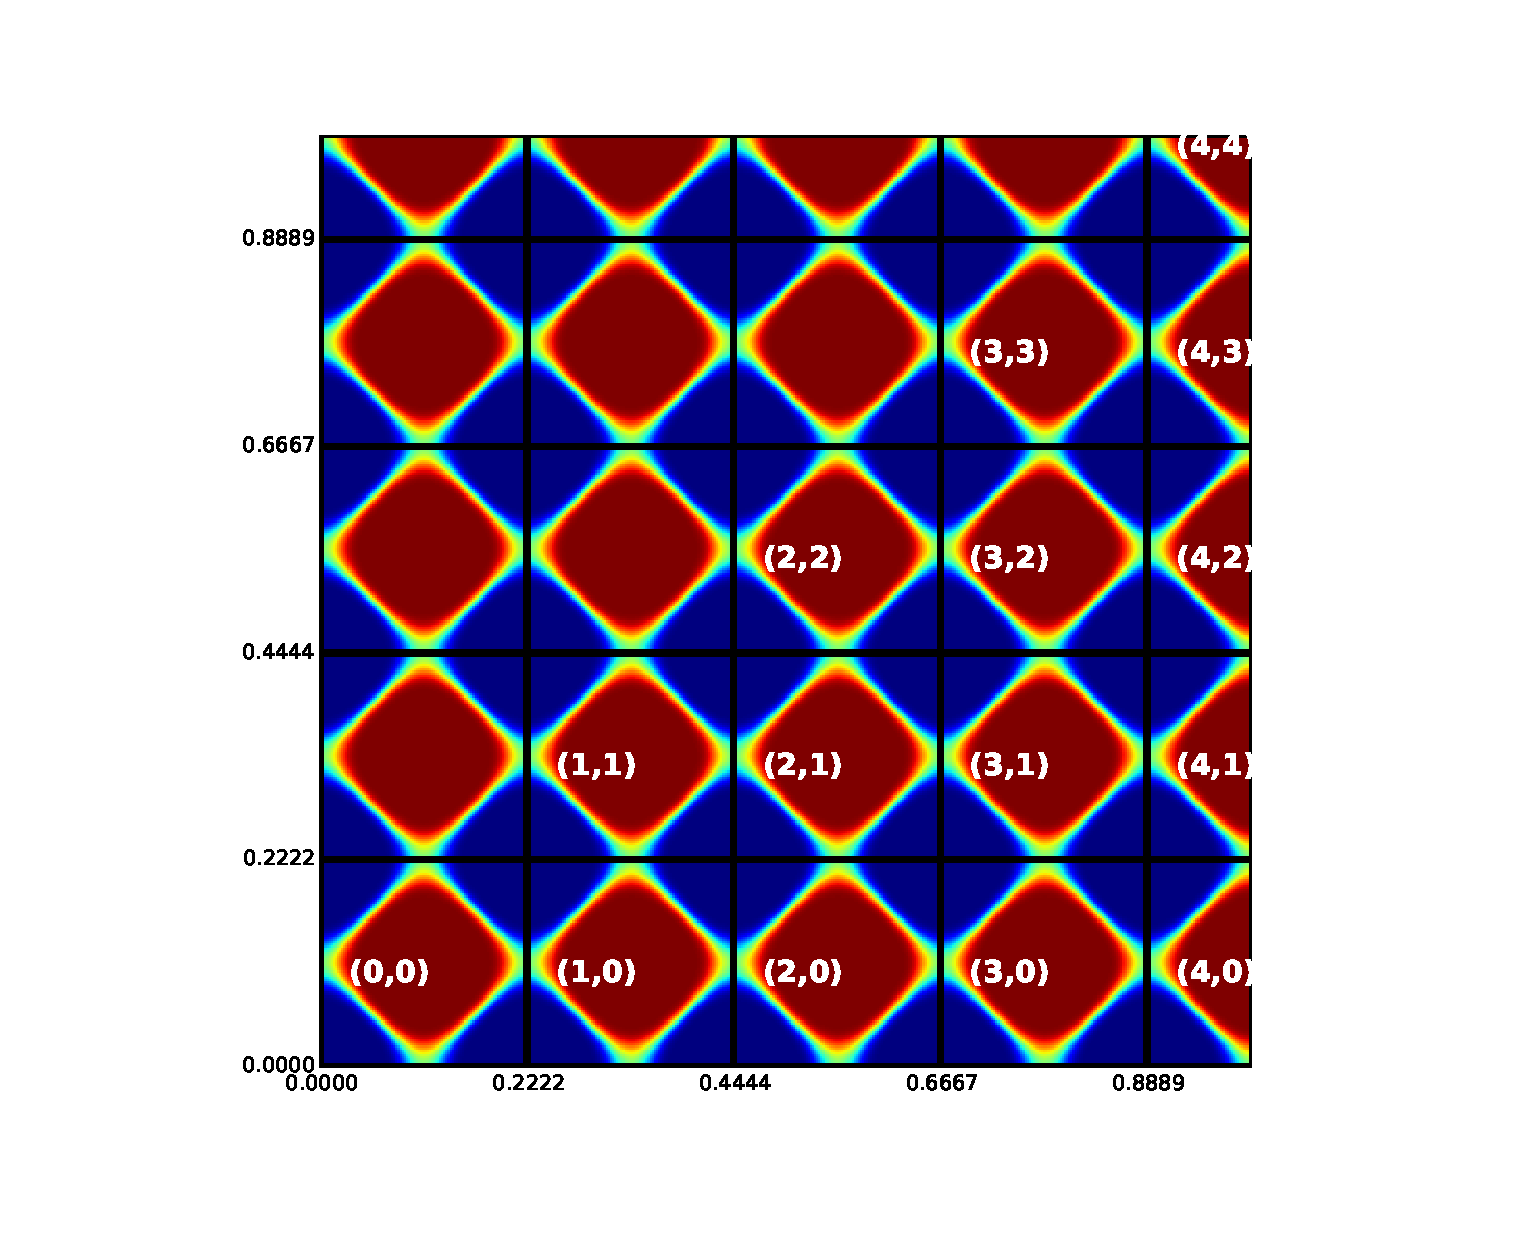
\includegraphics[width=\columnwidth]{figs/cells}
\caption{ \flabel{ic} 
Initial condition, $\phi(x,y,0,0)$, for 4.5 mode simulation.  
The bubbles are logically separated by the solid grid and each unique bubble is labeled.
}
\end{figure}

\begin{table}
\input{tbl/params.tbl}
\caption{ \tlabel{params}
Parameters of simulations.
The aspect ratio is defined with respect to the quiescent amplitude, $a_0$, from \eref{rollback}.
The last row is the simulation that extends the tank by a factor of two in the vertical direction.
}
\end{table}

Three simulations were conducted to reproduce experiments with 2.5, 3.5, and 4.5 modes across the diagonal.
Then, an extension of the 4.5 mode experiment with twice the vertical extent was performed.
Finally, a 4.5 mode calculation with periodic boundary conditions and unit Schmidt number was performed as a reference for comparing the growth of the bubbles in the wall-bounded flows.

The boundary conditions for the non-periodic simulations are no-slip for the velocity and no-flux (insulating) for the scalar.
The initial conditions for the velocity are quiescent.
The initial conditions for the scalar are the product of two cosines smeared by an error function in the z-direction:
\begin{equation}
  \phi(x,y,z,0) = \text{erf}\left[ \frac{z + a_0 \cos(k_x x) \cos(k_y y)}{\delta} \right] ,
\end{equation}
where $a_0$ is the initial amplitude,
$k_x$ and $k_y$ are the wave-numbers in the x and y directions, respectively, and
$\delta$ is the interface thickness.
In our case, $k_x = k_y$.
An example initial condition is plotted in \fref{ic}.
By symmetry, we know that the average scalar is zero, $H_{i,j} = H_{j,i}$, and that the spike dynamics are identical to the bubbles.

The Atwood number, local acceleration, and initial amplitude where taken from experimental measurements by Wilkinson and Jacobs~\cite{Wilkinson2007, JacobsPrivate}.
In the experiment, the interface has a non-zero initial velocity and the bulk flow is not measured.
Instead of trying to model the bulk flow, we used the linear theory, \eref{duff}, to transform the flow to quiescence.
Specifically, the system
\begin{align} \elabel{rollback}
H &= a_0 \cosh\left(\gamma (t - t_0)\right) \\
V &= a_0 \gamma \cosh\left(\gamma (t-t_0) \right)  \nonumber
\end{align}
where $H$ and $V$ were the experimental measures of the initial interface height and velocity, respectively,
is solved for $a_0$ and $t_0$, the quiescent amplitude and time.
The quiescent amplitude is used for the simulations.
The experiments to reproduce were selected such that solutions to \eref{rollback} existed and the bubble reached the greatest heights.

The viscosity is matched to the experimental fluids, but the diffusivity is not.
The Schmidt number in the experiments is in excess of 1000.
The computational cost of the simulation goes with the Schmidt number to the 4th power, so directly simulating such high Schmidt number was not possible.
Instead, the Schmidt number was varied in the range of 1 to 7 to gain a qualitative understanding of its influence on the flow.

It should be noted that, while the Atwood number was used to scale the local acceleration, the Boussinesq approximation implies that the Atwood number has been taken to zero while keeping the product $Ag$ fixed.
The generally accepted Boussinesq limit is $A = 0.05$, which is three times smaller than the Atwood number in this case.
Previous simulations directed at single-mode re-acceleration have been performed at $A \ge 0.15$, so it is not known whether re-acceleration persists in the limit as $A \rightarrow 0$.

The three simulations reproducing experimental runs are conducted on the Mira supercomputer at Argonne Leadership Computing Facility (ALCF).
The resolution and time-step was chosen to numerical stability constraints: a $256\times256\times512$ mesh of 7th order elements for 11,509,170,176 degrees of freedom.
The simulation was distributed over 524,288 cores and 1,048,576 MPI processes.
64 outputs were written to disk, each 6/8ths of a TiB.
The number of elements and degrees of freedom are doubled for the extension to twice the vertical extent.

\subsection{Post-processing}
The simulation outputs the velocity, pressure, and scalar fields at the Gauss-Lobatto-Legendre points in double precision.
They are post-processed into low-dimensional observables: the bubble height and two-dimensional slices of the velocity, vorticity, pressure, and scalar through the horizontal mid-plane and vertical diagonal.
Post-processing is performed using the `nek-analyze' post-processing framework, which implements a MapReduce-like backend for parallel, out-of-core analysis.

The bubble height is defined as:
\begin{equation} \elabel{h_exp}
H = \sup \left\{ z : \min_{x,y} \phi(x,y,z) < 0\right\},
\end{equation}
which, avoids measuring the diffusive growth by tracking the center of the interface profile instead of the ends.
The bubble velocity is found by fitting a cubic spline to $H(t)$ and differentiating.

The height of individual bubbles, $H_{i,j}$, is found by restricting $\min_{x,y}$ in \eref{h_exp} to the span-wise square of diagonal length $\lambda$ centered on the bubble in the $i$-by-$j$-th position.
The bubble domains and labels are shown in \fref{ic}.



\section{Results} \slabel{results}

\subsection{Validation}

\subsubsection{Linear growth rate}

\begin{table}
\input{tbl/linear.tbl}
\caption{ \tlabel{linear}
Growth rate: linear theory vs simulation.
Theoretical values are calculated as in \eref{duff}.
Simulation values are calculated as in \eref{linear_sim}.
The aspect ratio is shown for the second sample, $h_1 / \lambda$.
Note the difference in Schmidt number between the two $4.5$ mode cases.
}
\end{table}

We compute the growth rate from the bubble height at the first simulation output time:
\begin{equation} \elabel{linear_sim}
\gamma \approx \frac{1}{t_1} \text{acosh}\left(\frac{h(t_1)}{h(0)}\right), 
\end{equation}
and collect the results in \tref{linear}.
Because the simulations targeted the non-linear regime, the height is not available until characteristic time $\tau = t \gamma \sim 2$ and aspect ratio $h / \lambda \approx 0.1$.
Therefore, we expect the simulation value to be below the theoretical value given by \eref{duff} due to saturation.

The agreement is good, with only the lower Grashof, higher aspect ratio 4.5 mode calculation deviating more than a part in one hundred.
The 2.5 mode simulation outperforms the theory slightly.
This could be due to the long-wavelength finite size effect discussed later, which is stronger for fewer modes in the finite domain.

\subsubsection{Froude number}

\begin{figure}
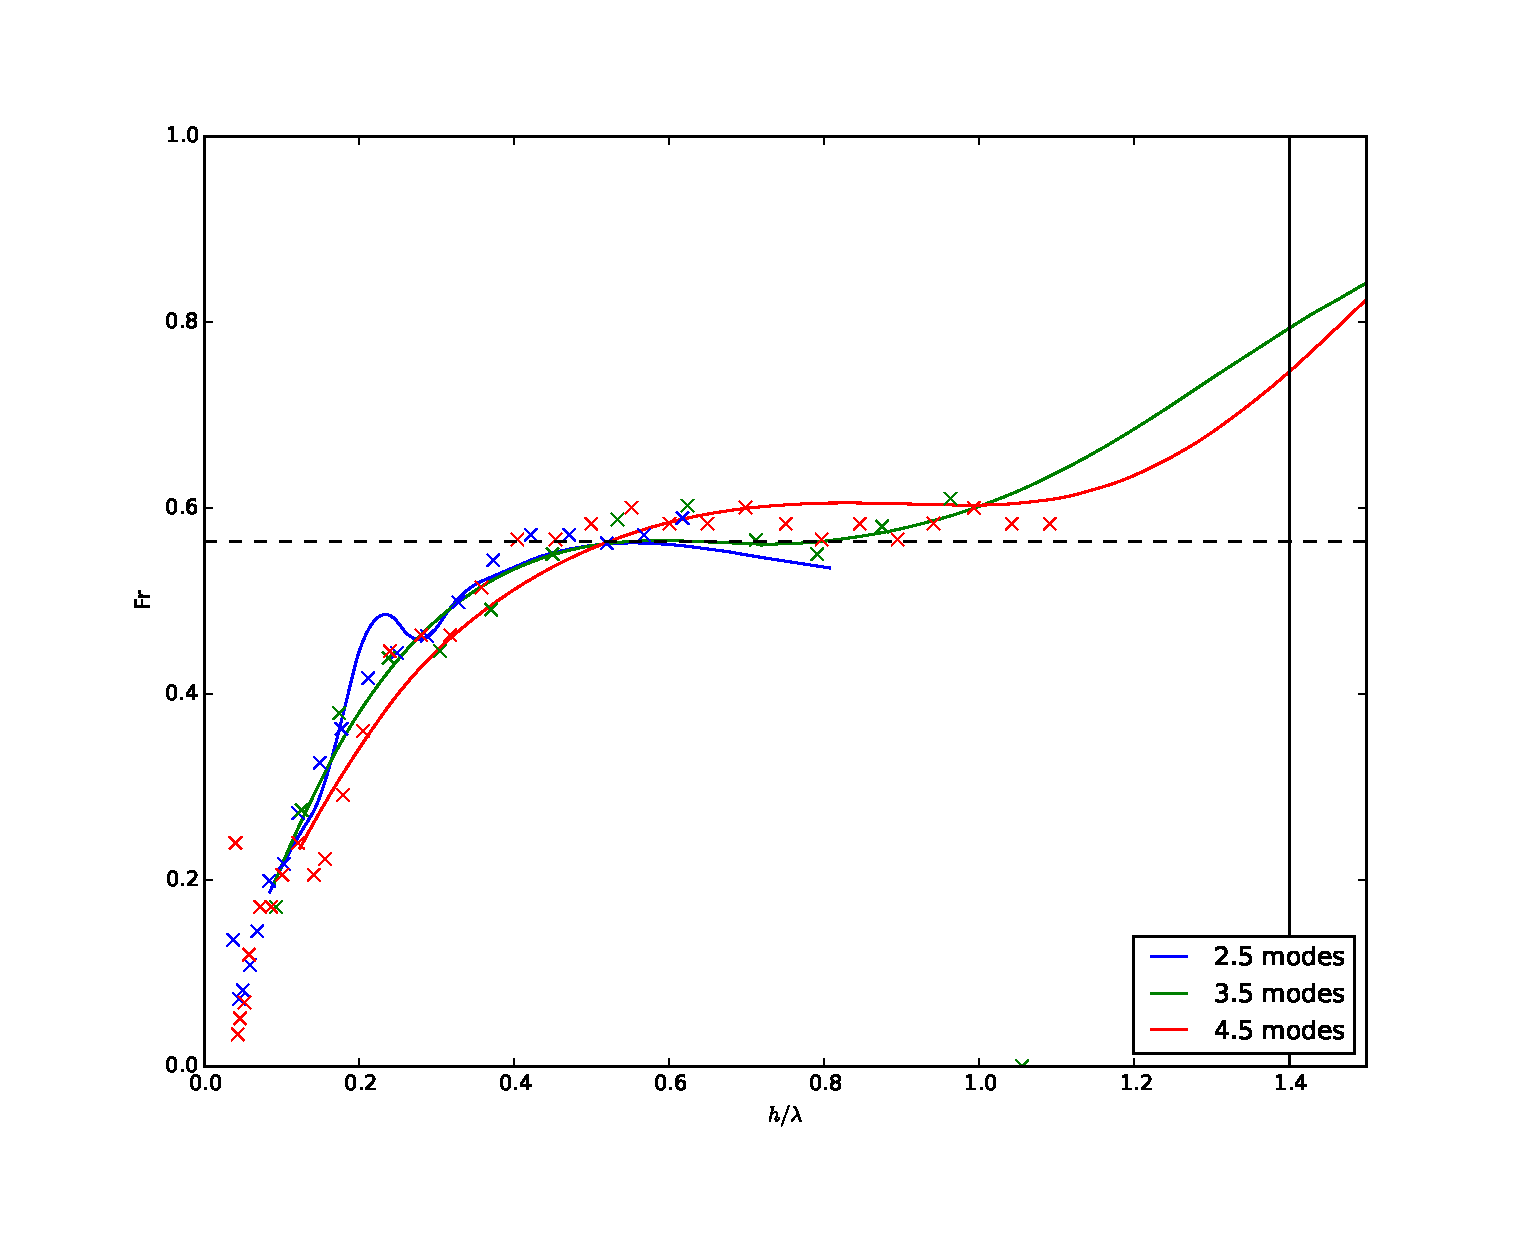
\includegraphics[width=\columnwidth]{plts/Fr}
\caption{ \flabel{froude} 
Froude number vs height, non-dimensionalized by the wavelength.
Lines are the derivative of cubic splines through simulation outputs.
Points are from experiment via direct measurement of the bubble velocity~\cite{JacobsPrivate}.
The dotted horizontal line is positioned at Goncharov's theoretical value of $\pi^{-1/2}$~\cite{Goncharov2002}.
}
\end{figure}

\begin{figure}
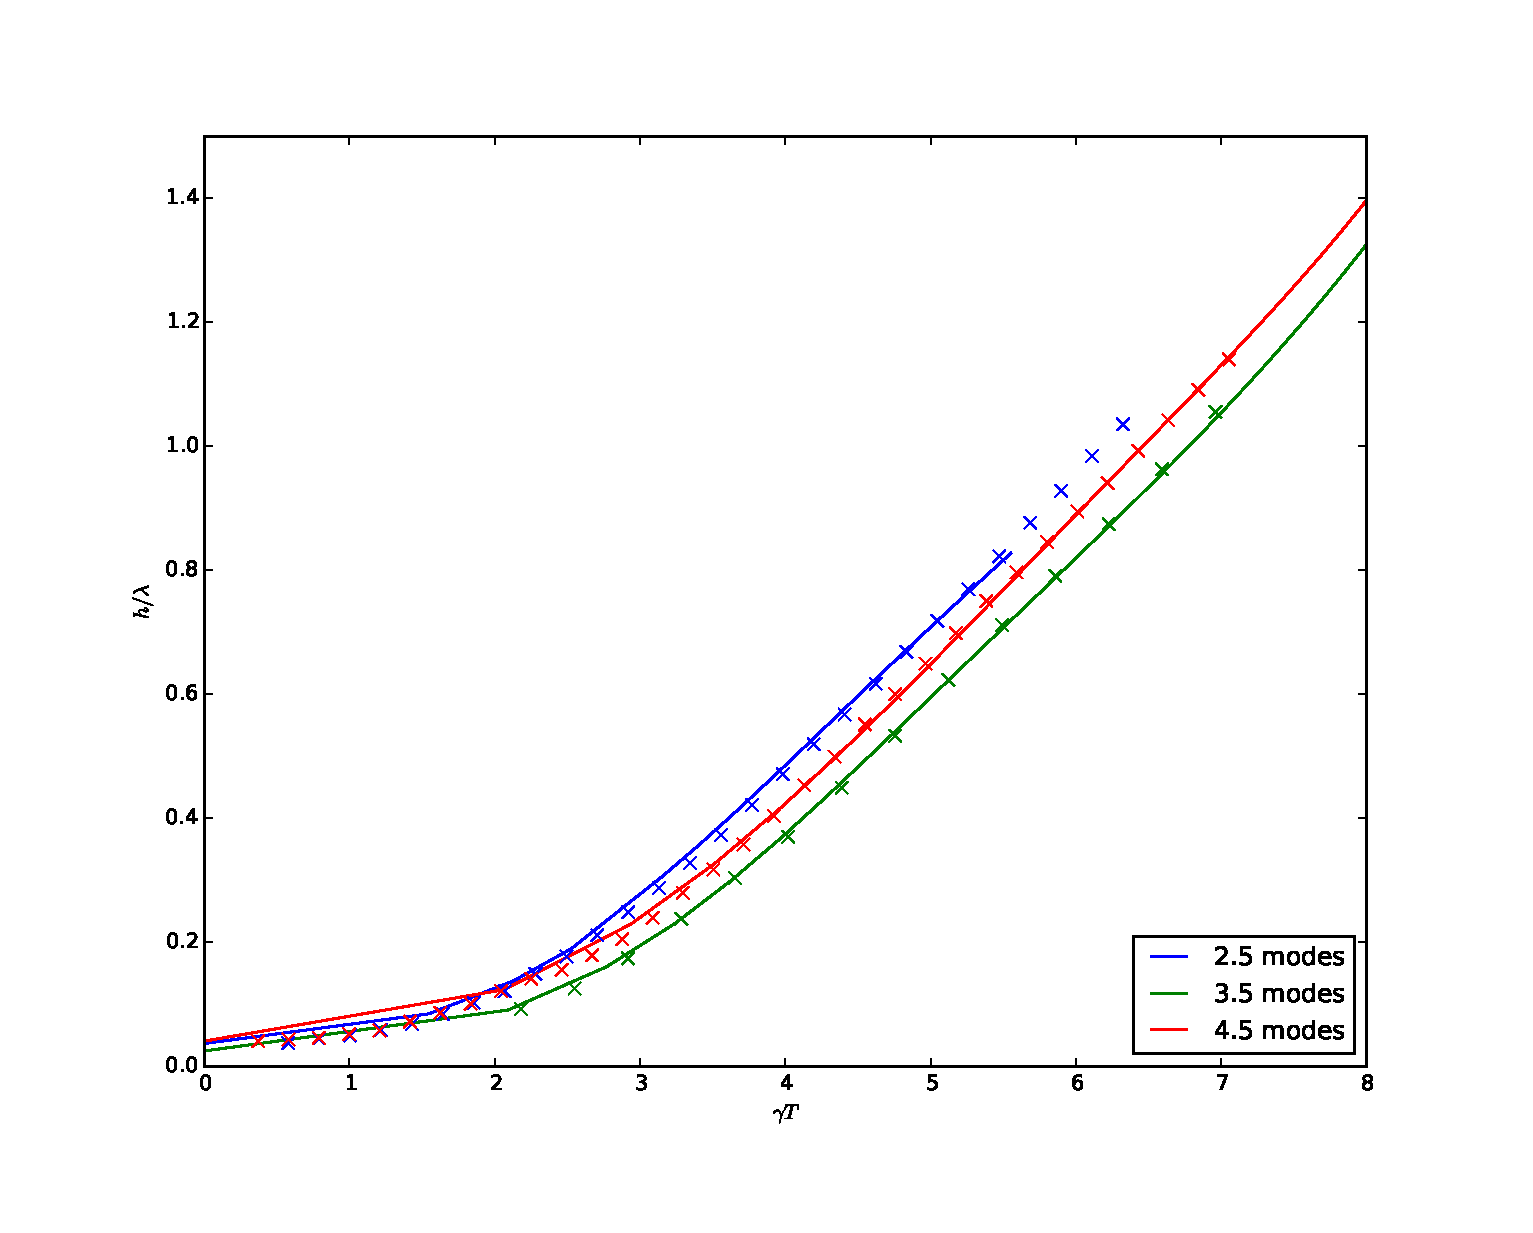
\includegraphics[width=\columnwidth]{plts/aspect}
\caption{ \flabel{aspect} 
Bubble height vs time, non-dimensionalized by the wavelength and linear growth rate, respectively.
Lines are cubic splines through simulation outputs.
Points are from experiment~\cite{JacobsPrivate}.
The points are shifted in time to minimize the square deviation from the spline summed over the plotted points.
}
\end{figure}

The experiments observe only the diagonal plane and measure the height with respect to the most internal bubble.
Therefore, we plot in \fref{froude} the non-dimensional velocity, i.e. the Froude number, of the central bubble alone:
\begin{equation}
	\text{Fr} = \frac{v}{\sqrt{ A g \lambda}}
\end{equation}
In each case, the simulation exhibits the same qualitative behavior as the experiment:
exponential growth saturating to a stagnation velocity around Goncharov's theoretical value of $\text{Fr} = \pi^{-1/2}$~\cite{Goncharov2002}.
In cases where the simulation and experimental data extend in time, the beginnings of re-acceleration are also seen.

The 2.5 mode case exhibits peculiar behavior with two inflection points around aspect ratio $h / \lambda = 0.2$.
This is not an issue with the splines, as can be seen in \fref{aspect}, which plots the non-dimensional height vs non-dimensional time without splines.
The 2.5 mode case, which has the highest Grashof and Schmidt numbers, went unstable.
Upon inspection, the 5\% filtering was unable to suppress the oscillations in the scalar field.
This simulation could be retried with greater resolution, but, given the stability of the 3.5 mode case, the computational cost would be up to 43$\times$ greater, which is why it was not repeated in this study.

\subsection{Extension}

Given the agreement between the simulations and the experiment, we can use the simulations to explore the flow in ways that are not readily accessible experimentally.
In this study, we extend the subject cases and analysis in three ways.
First, we calculate the height of each bubble in the tank individually and use the results to study finite size effects.
Second, we extend the 4.5 mode experiment by a factor of two in the vertical extent of the domain and simulation time to delay interaction with the top boundary and reach later times and larger bubble heights.
Finally, we consider the span-wise, vs stream-wise, flow by taking slices of the midplane and observing pressure driven secondary flows.
These three extensions are a small sample of the types of observations that are available numerically.

\subsubsection{Wall effects}

\begin{figure*}
\begin{subfigure}[b]{\columnwidth}
  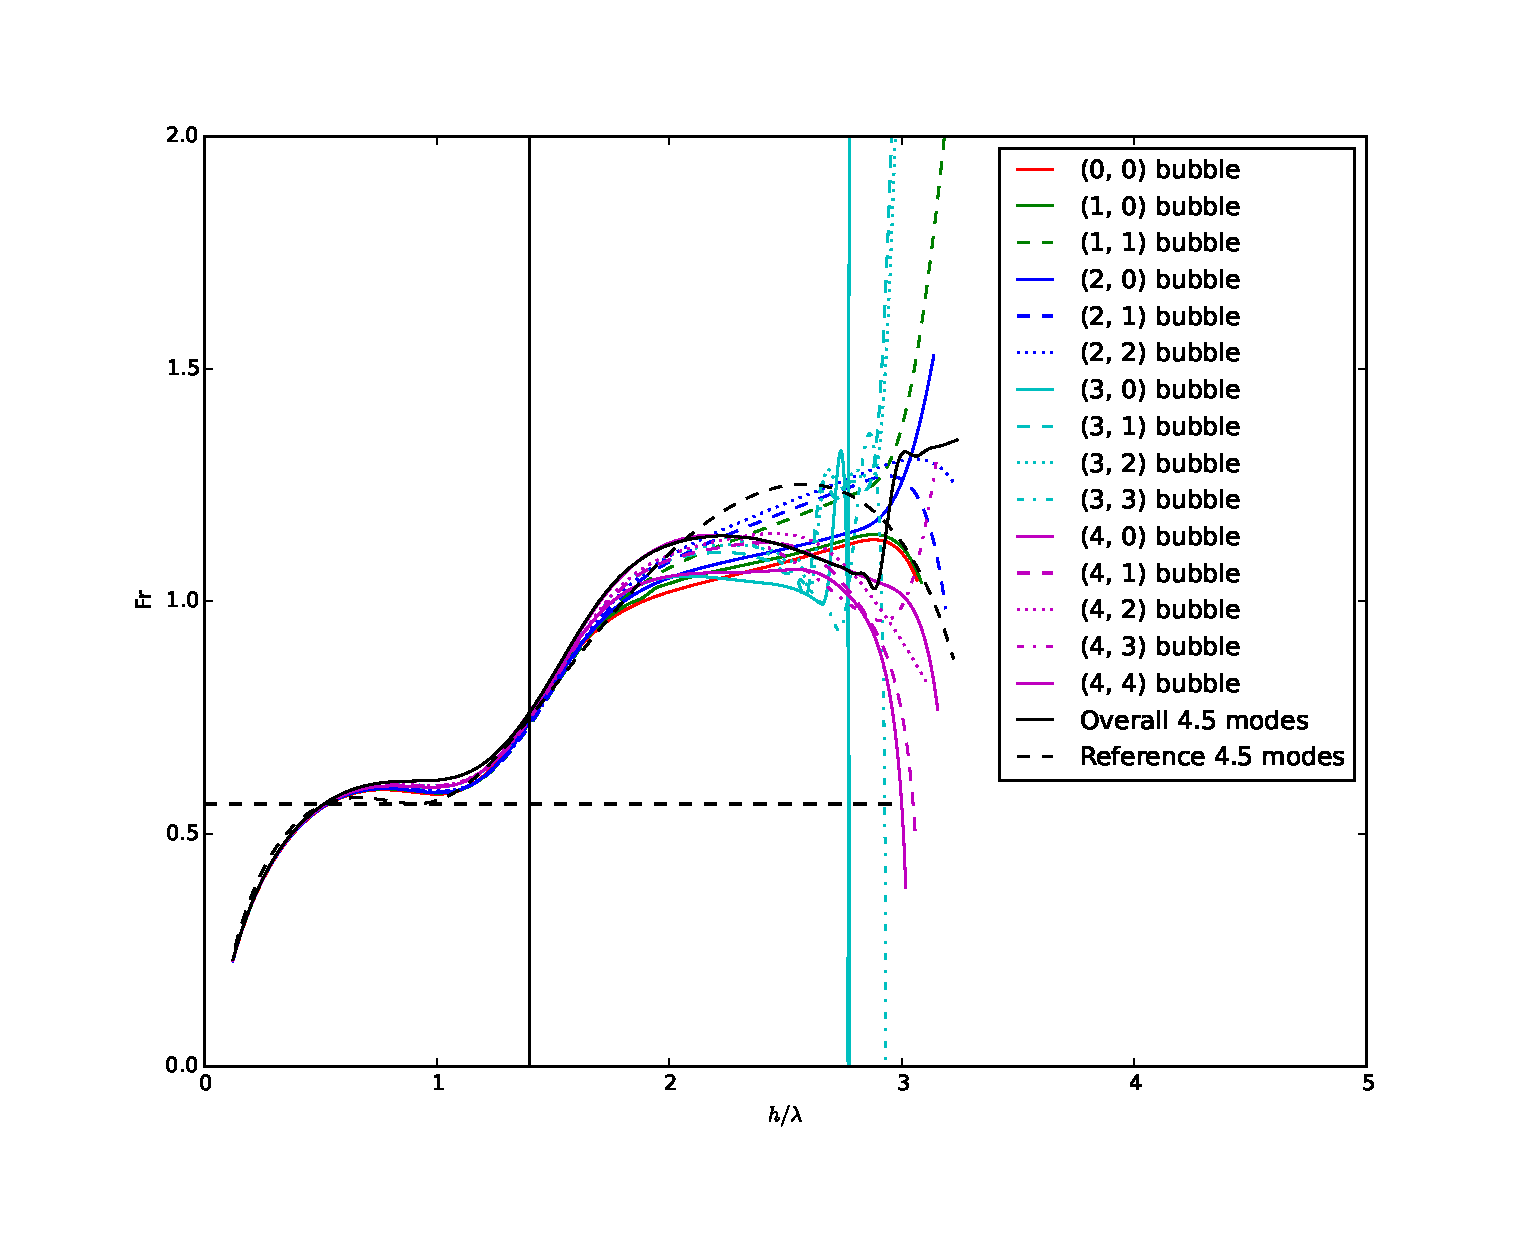
\includegraphics[width=\columnwidth]{plts/walls_Fr}
\end{subfigure}
\begin{subfigure}[b]{\columnwidth}
  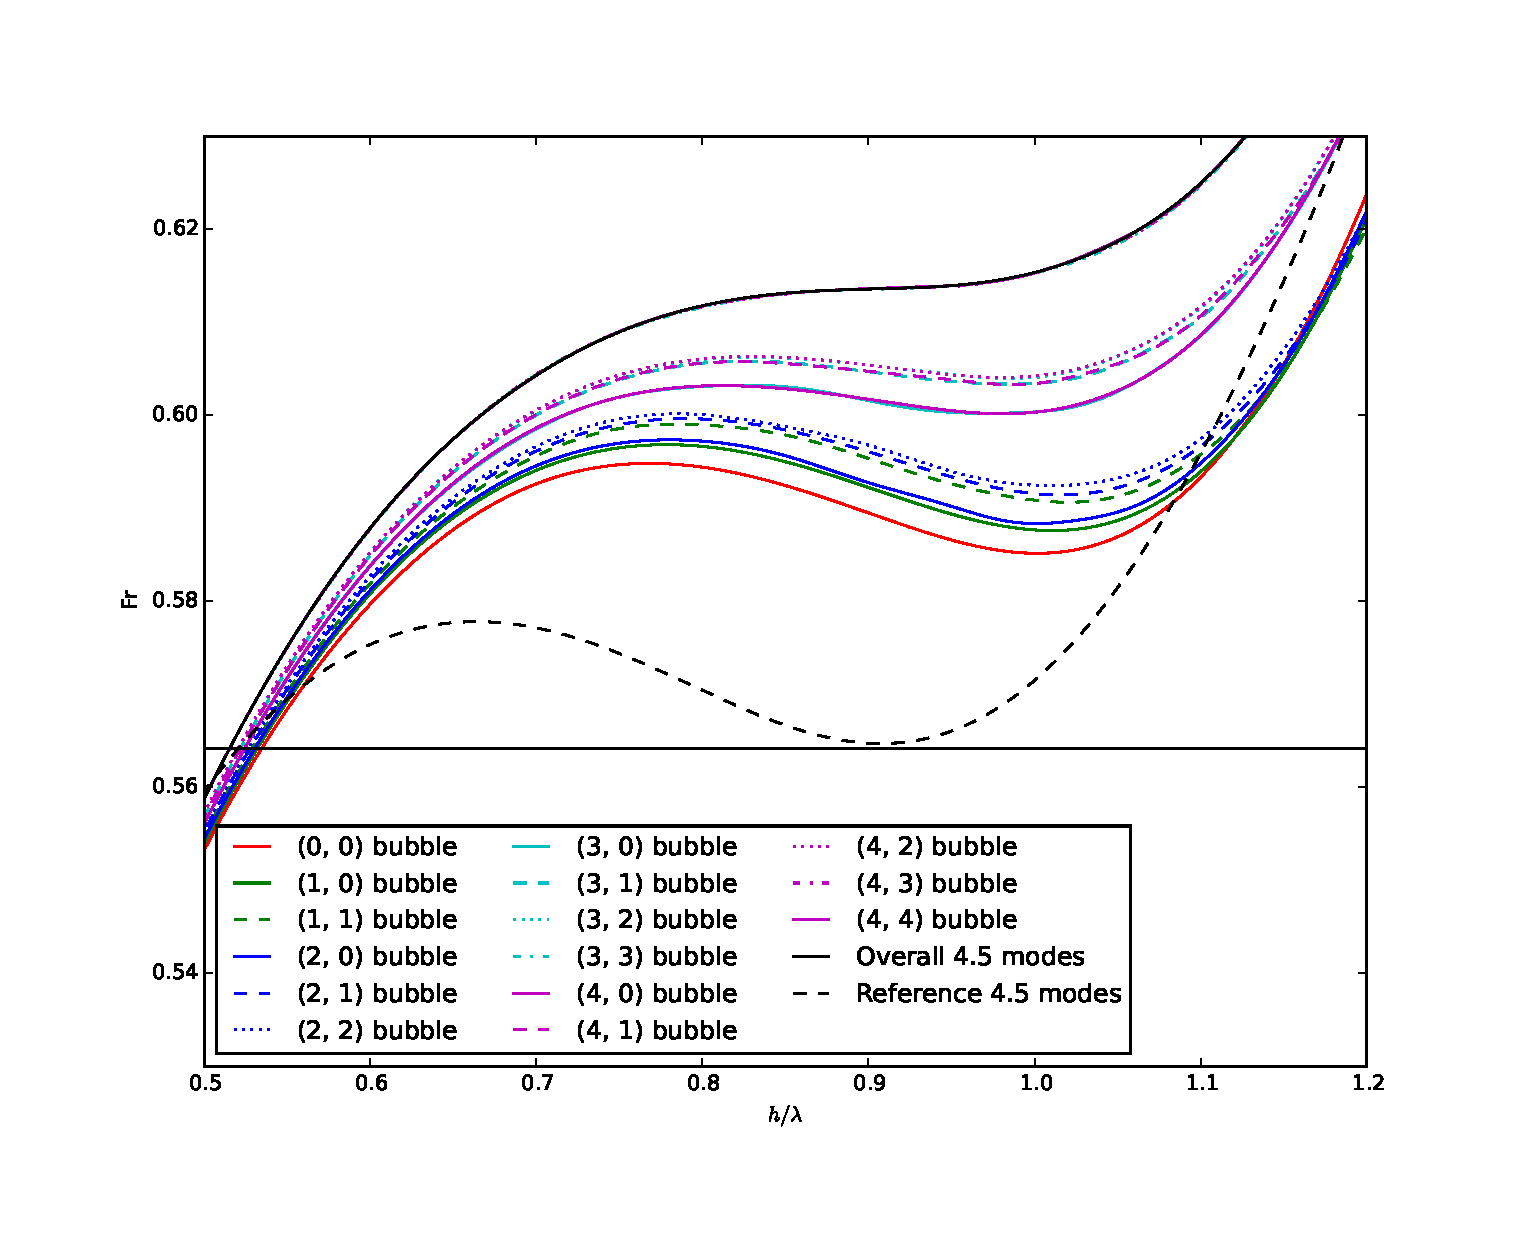
\includegraphics[width=\columnwidth]{plts/walls_Fr_zoom}
\end{subfigure}
\caption{ \flabel{froude_wall} 
Froude number as a function of height, non-dimensionalized by the wavelength, by bubble in the 4.5 mode simulation.
Solid line is from the height defined as the maximum taken over the entire span-wise domain.
Dotted line is the periodic reference calculation.
}
\end{figure*}

\begin{figure*}
\begin{subfigure}[b]{\columnwidth}
  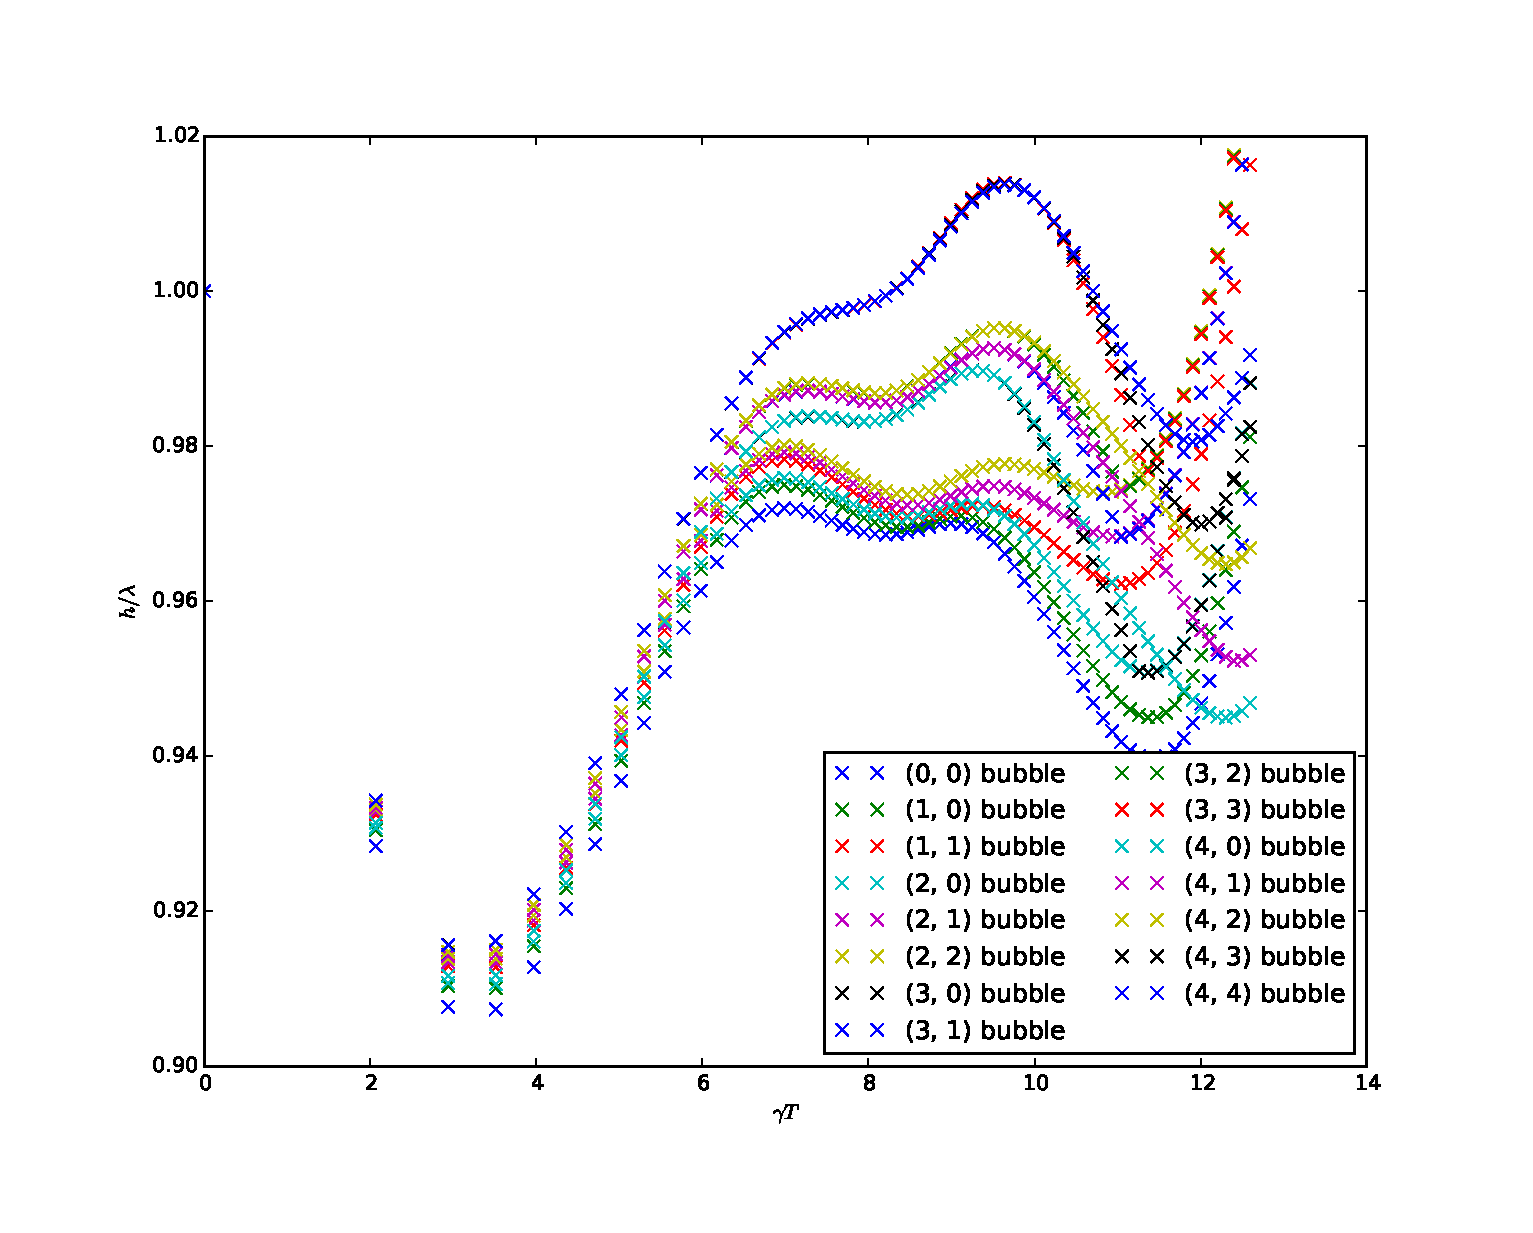
\includegraphics[width=\columnwidth]{plts/walls_h}
\end{subfigure}
\begin{subfigure}[b]{\columnwidth}
  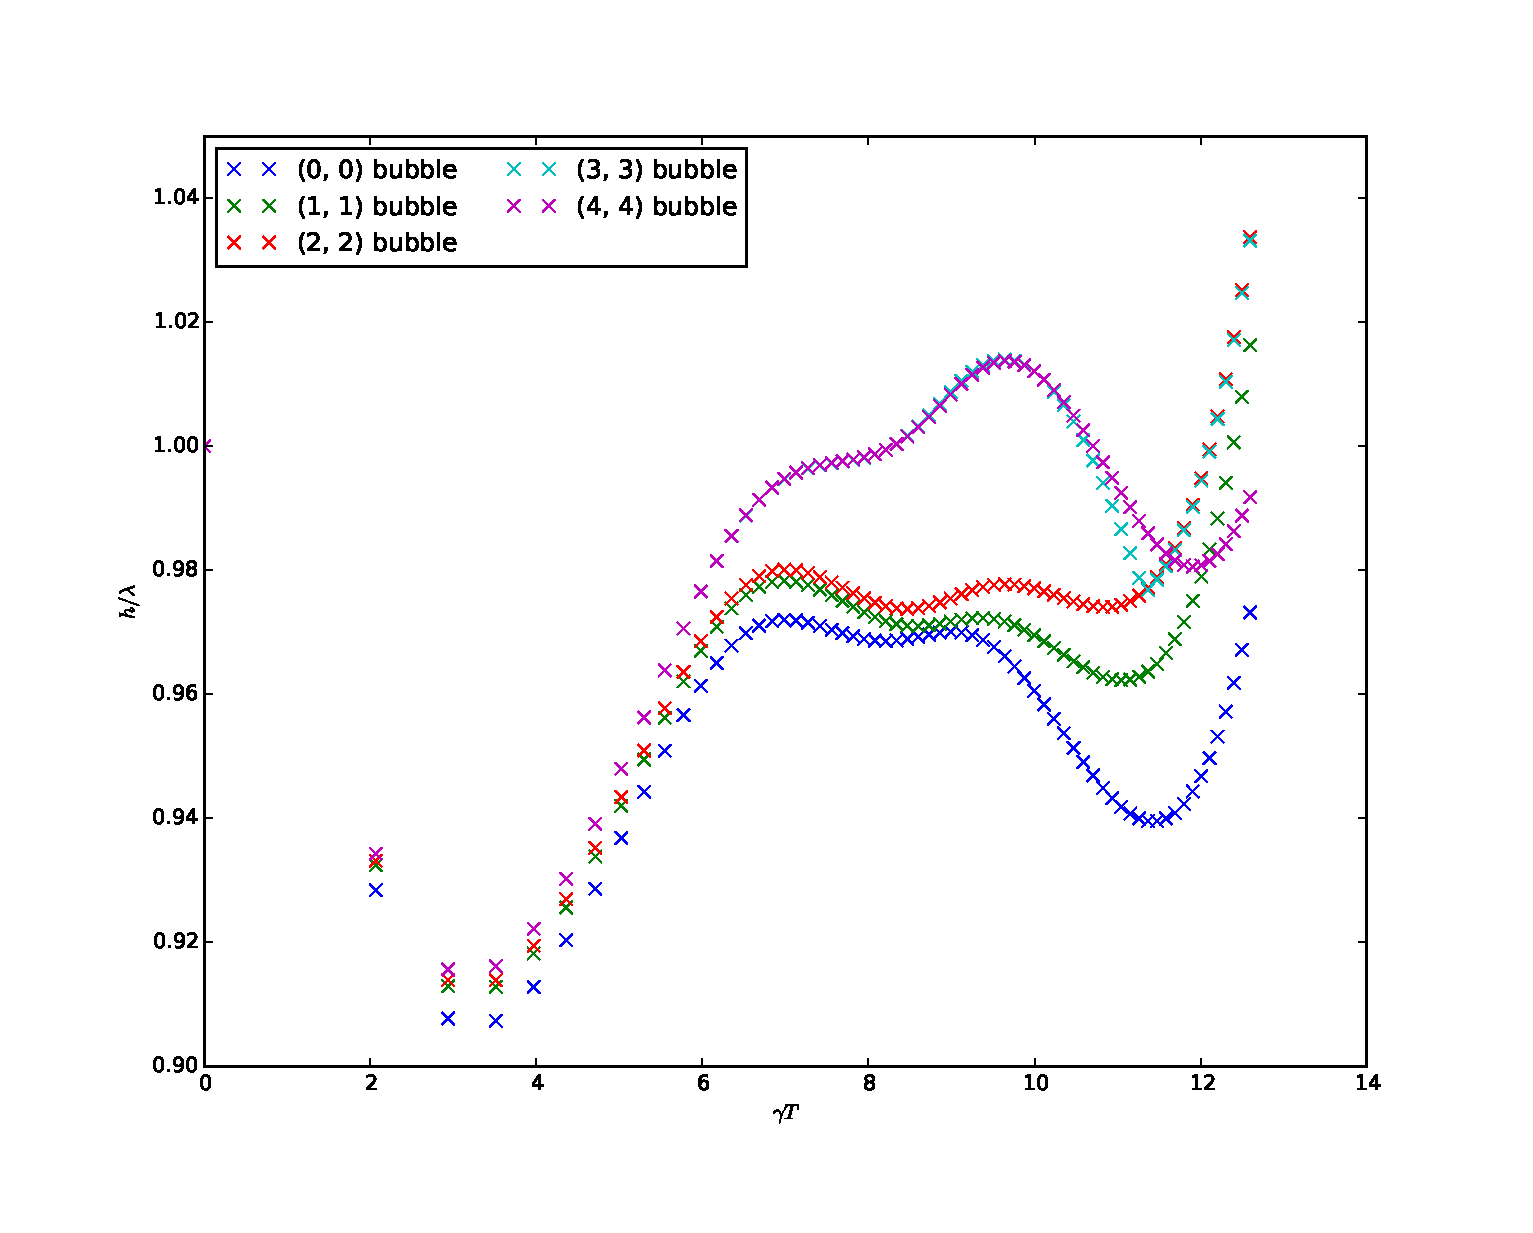
\includegraphics[width=\columnwidth]{plts/walls_h_diag}
\end{subfigure}
\caption{ \flabel{ratio_wall}
Ratio of wall-bounded bubble height to periodic bubble height in the 4.5 mode simulation.
}
\end{figure*}

\begin{figure*}
\begin{subfigure}[b]{0.66\columnwidth}
  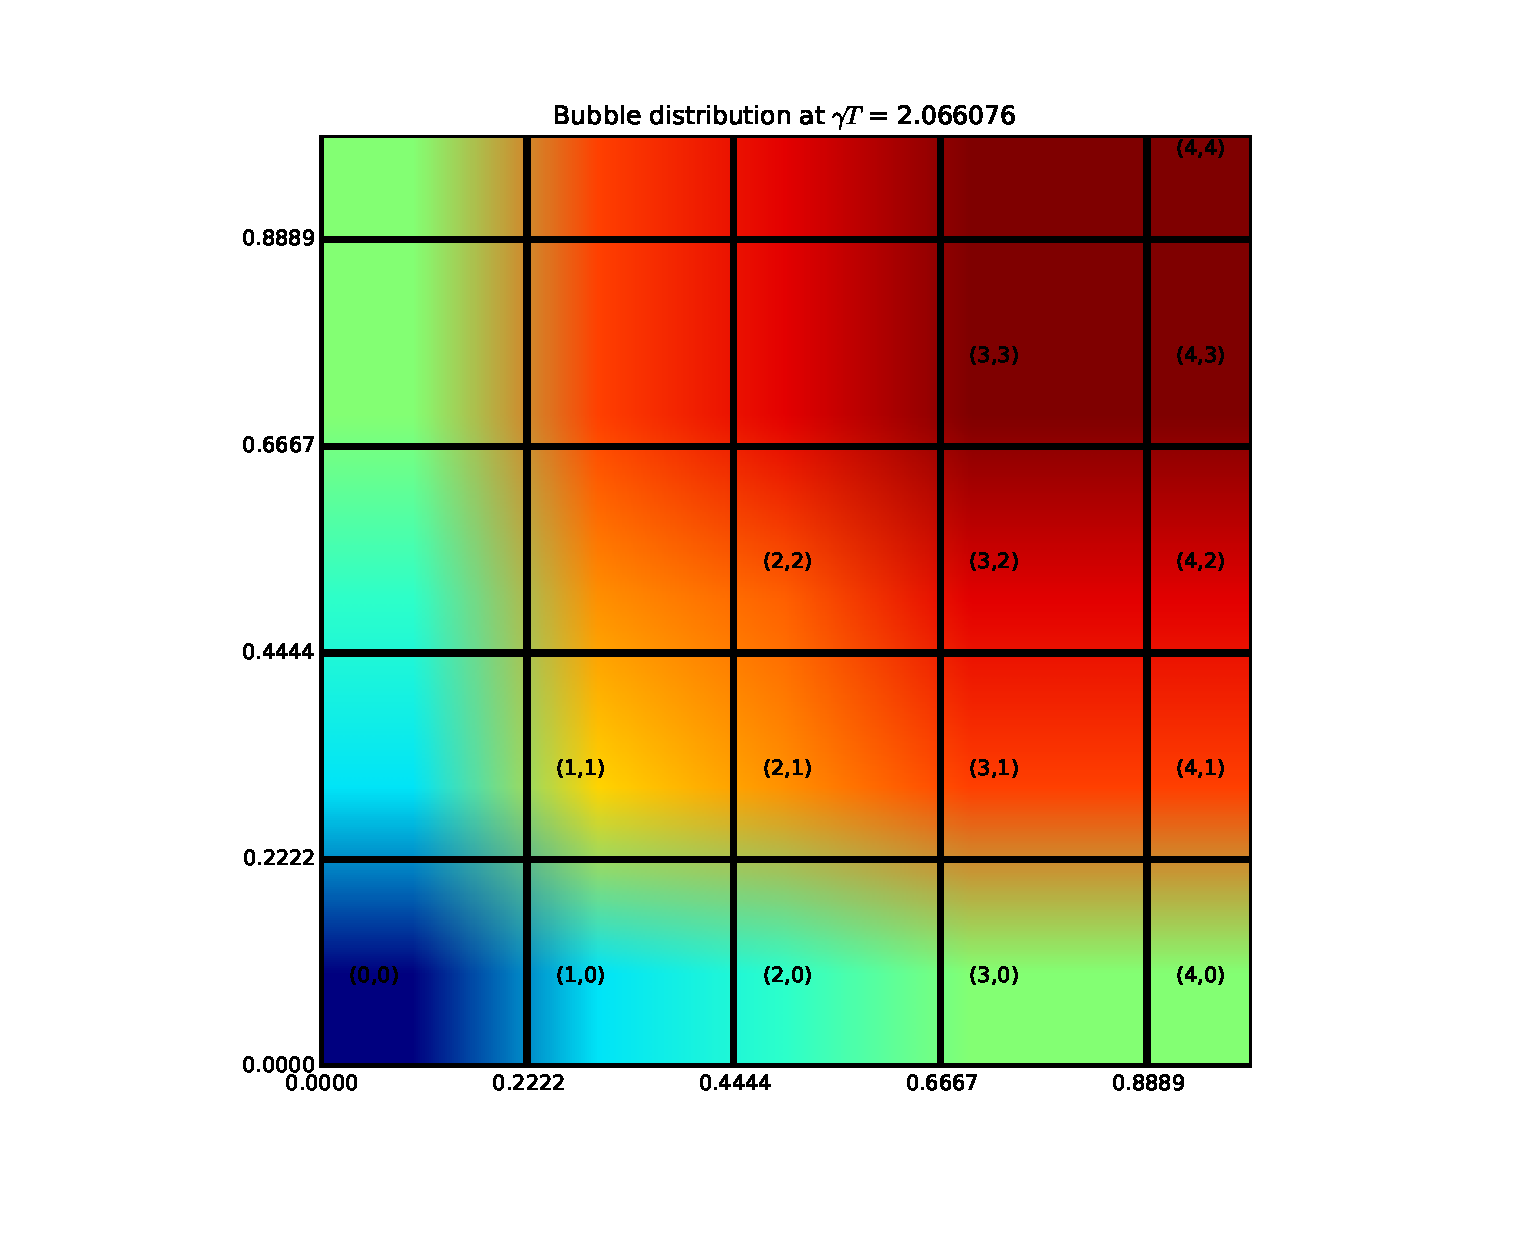
\includegraphics[width=0.66\columnwidth]{figs/spatial_bubble-1}
\end{subfigure}
\begin{subfigure}[b]{0.66\columnwidth}
  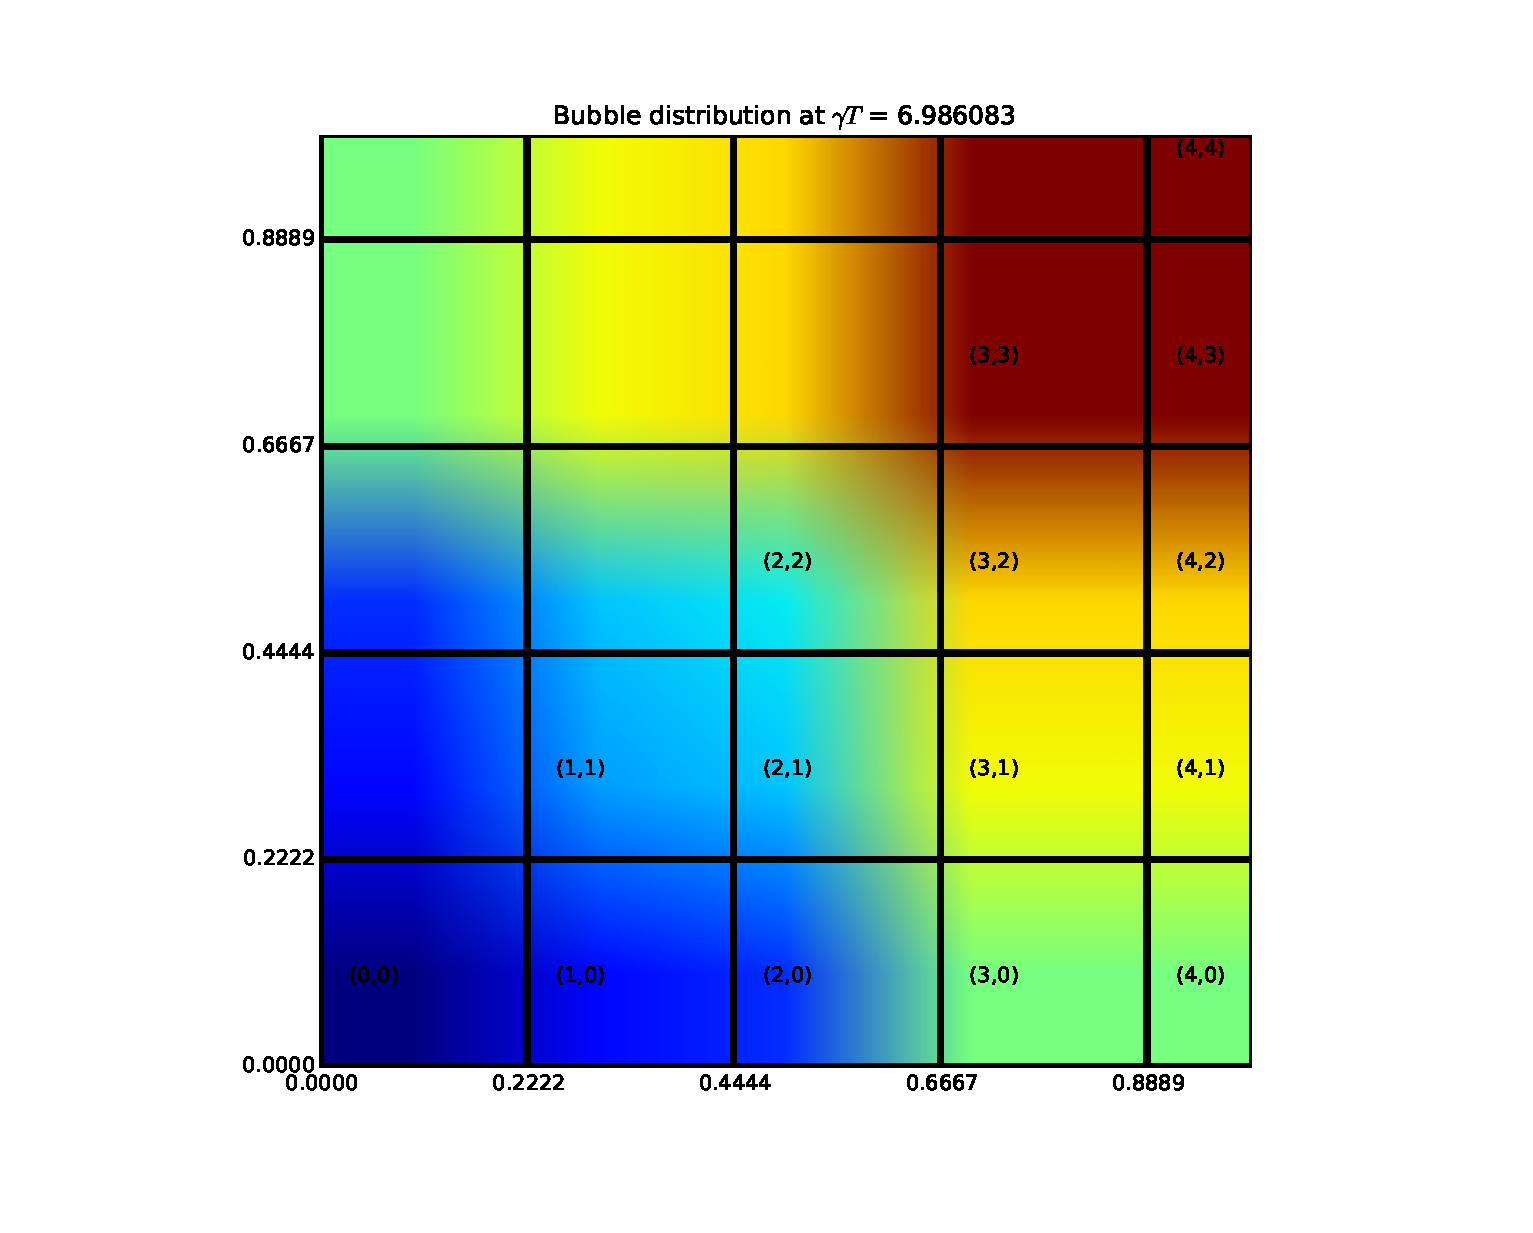
\includegraphics[width=0.66\columnwidth]{figs/spatial_bubble-17}
\end{subfigure}
\begin{subfigure}[b]{0.66\columnwidth}
  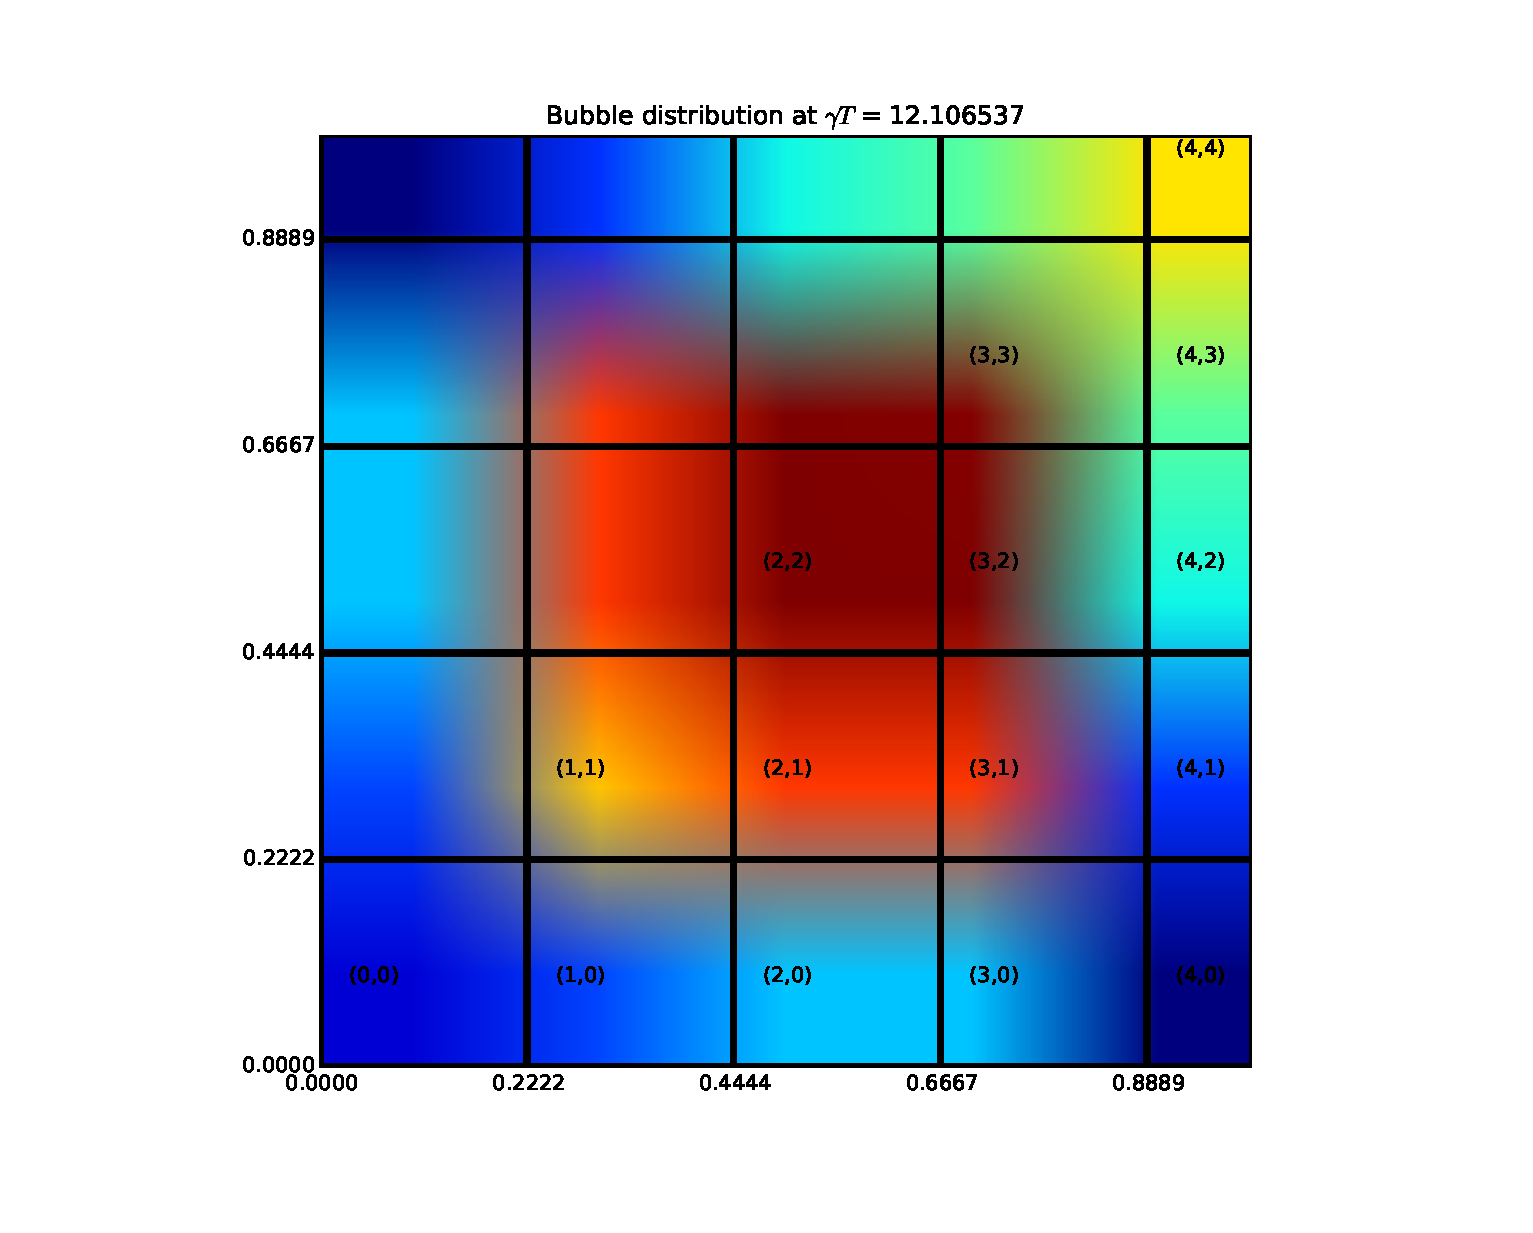
\includegraphics[width=0.66\columnwidth]{figs/spatial_bubble-59}
\end{subfigure}
\caption{ \flabel{bubble_slice}
Spatial distribution of bubble heights at three times.
The first time corresponds to the minimum in \fref{ratio_wall}, which is during the transition from linear to non-linear growth
The second time is taken from the stagnation phase.
The third time is taken from the end of the simulation when the central bubbles are squeezed by the growing boundary layer.
}
\end{figure*}

The individual bubble heights for the $4.5$ mode case are computed as in \eref{h_exp}, but restricted to the span-wise domain nearest to the bubble tip, which is marked in \fref{ic}.
The bubble Froude numbers are plotted in \fref{froude_wall}, alongside the aggregate and purely periodic values.

There are at least three mechanisms by which the walls divert the flow from its fully-periodic preference.
The first is that the no-slip boundaries that pass along the diagonal of the boundary bubbles and spikes create a boundary layer that viscously damps vertical flow.
The second is that the pressure gradient from the boundary layer pushes the boundary bubbles and spikes towards the interior of the domain.
These two effects have been studied independently in the context of multi-phase bubbles rising near walls~\cite{Takemura2002}, and are characterized as wall drag and lift forces.
Finally, the finite nature of the span-wise lattice of bubbles and spikes, coupled with the vertical symmetry condition that the total bubble volume must equal the total spike volume, breaks one of the 4-fold symmetries of the infinite cubic lattice causing a local aggregation of spikes in the $(0,0)$ corner and of bubbles in the $(4,4)$ corner.
The local aggregation sets up one low-amplitude long-wavelength mode across the diagonal.

These three mechanisms promote and penalize the growth of different bubbles in the finite lattice, allowing us to infer the relative magnitudes of the effects based on the performance of the bubbles compared to their periodic counterparts.
The wall drag penalizes the growth of bubbles that contain a boundary: the bubbles in the 4th column.
Because the effect also penalizes the growth of the spikes that contain boundaries, it should encourage the growth of the bubbles adjacent to those spikes: those in the 0th row.
The effect should alternate and diminish towards the interior of the domain.
The wall lift pushes bubbles and spikes at the boundary towards the interior.
This reduces the form drag on the interior bubbles by increasing the pressure on their trailing edges.
When adjacent bubbles actually touch, skin drag is also reduced.
Overall, wall lift promotes the growth of the interior bubbles.
Finally, the long-wavelength mode promotes growth of bubbles in the bubble heavy corner and penalizes growth of bubbles in the spike heavy corner.

The spatial distribution of the bubble heights can be seen in \fref{bubble_slice} and the heights relative to the periodic bubble can be seen in \fref{ratio_wall}.
At moderate times, the $(4,4)$ bubble leads and the $(0,0)$ bubble trails, indicating that the long-wavelength mode due to symmetry breaking is the dominant effect.
Additionally, all of the bubbles under-perform their periodic counterpart, indicating that the wall drag has damped the overall flow but with less spatial dependence than the long-wavelength mode.
At late times, the central $(2,2)$, $(2,1)$  bubbles are accelerated while the edge bubbles break down, indicating the growing importance of the wall lift effect.
The wall lift ultimately leads to bubble collisions that destroy the bubble lattice, enhance mixing, and break down the flow.

\subsubsection{Late-time behavior}

\begin{figure*}
\begin{subfigure}[b]{\columnwidth}
  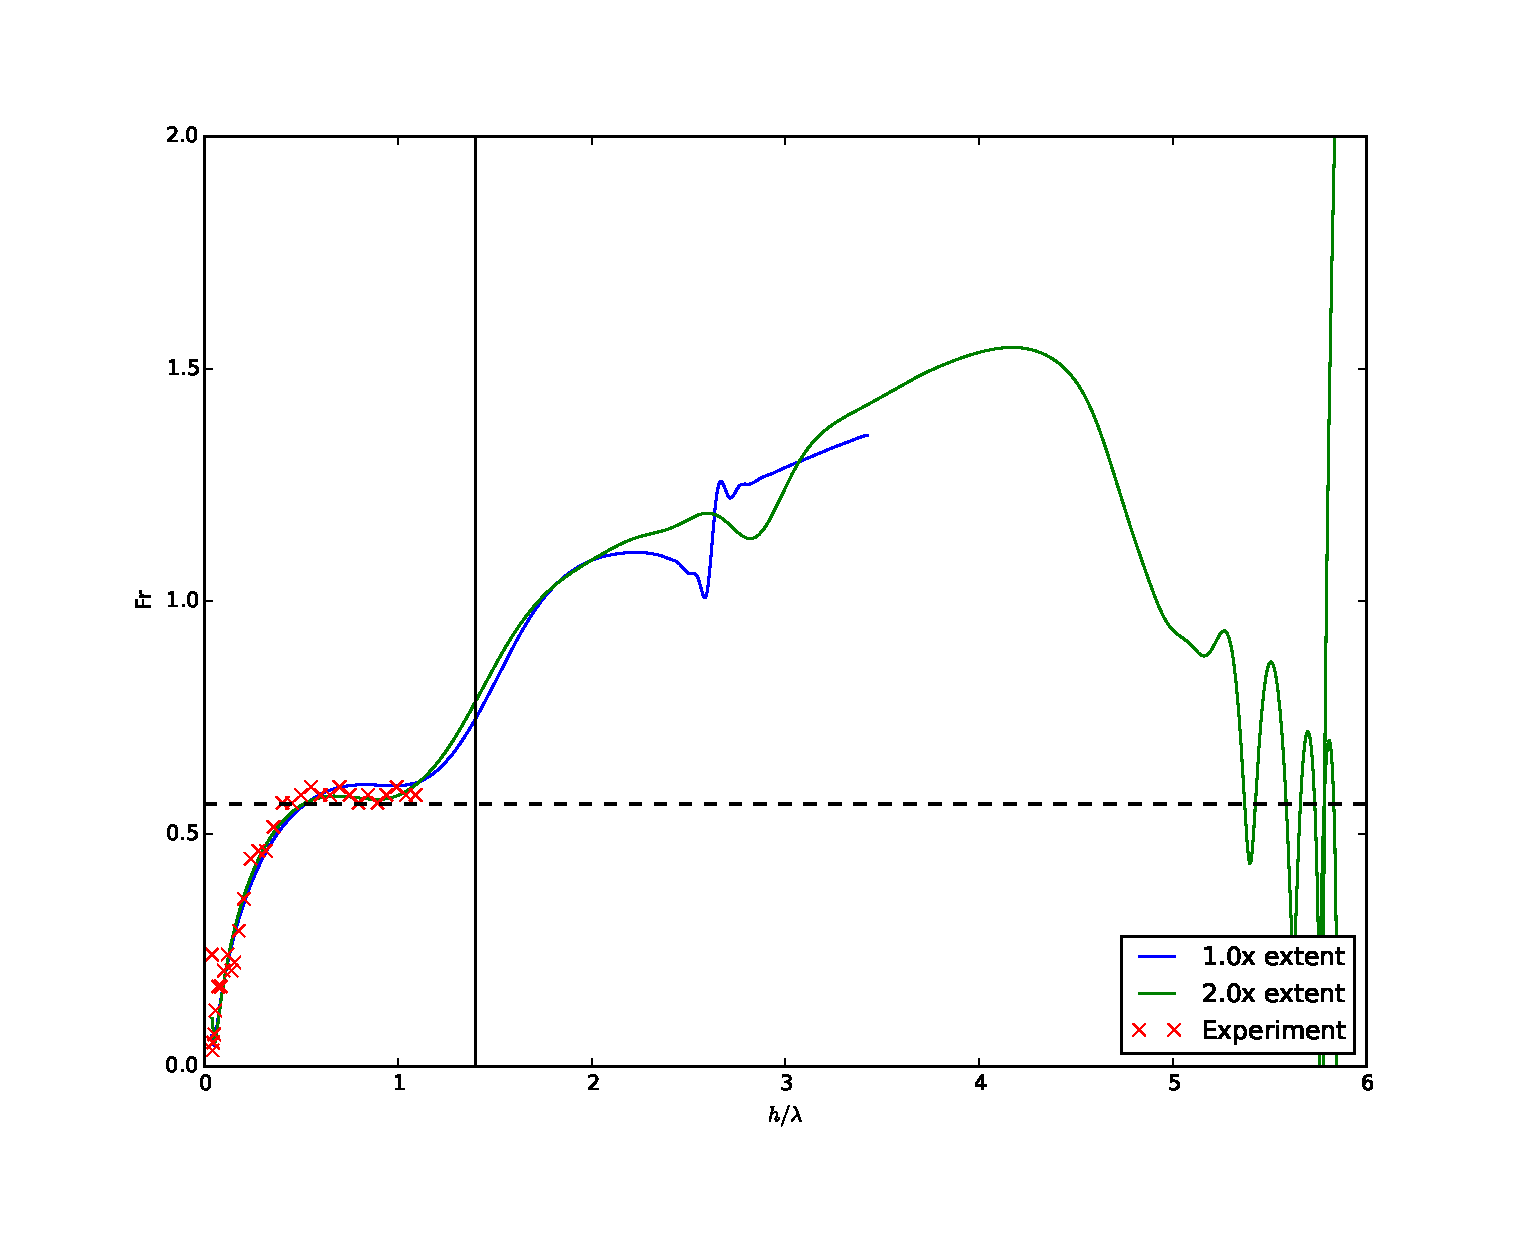
\includegraphics[width=\columnwidth]{plts/Fr_long}
\end{subfigure}
\begin{subfigure}[b]{\columnwidth}
  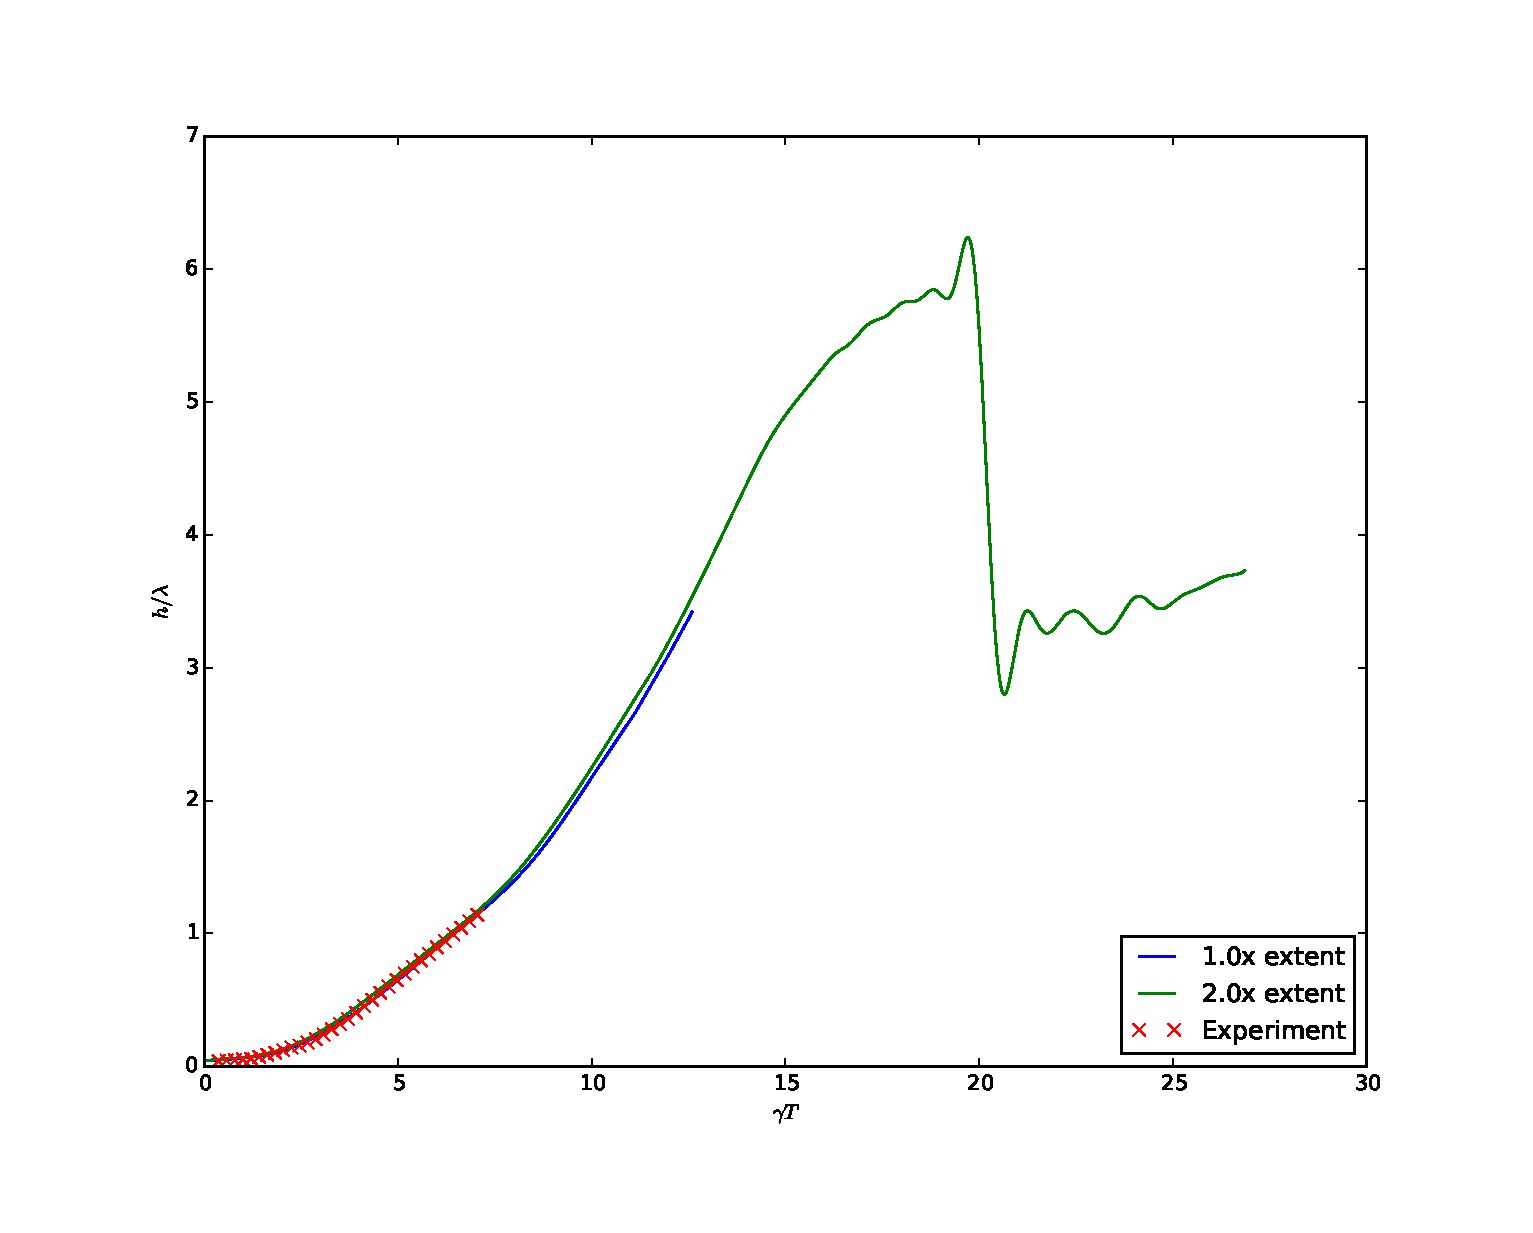
\includegraphics[width=\columnwidth]{plts/aspect_long}
\end{subfigure}
\caption{ \flabel{long_dynamics}
Bubble velocity and bubble height vs time, non-dimensionalized by the wavelength and linear growth rate, for 4.5 mode simulations and experiment.
Lines are from simulation output, one case with the same vertical extent as the simulation and in the other with twice that vertical extent.
Points are from experiment via direct measurement of the bubble velocity and bubble height.
The dotted horizontal line is positioned at Goncharov's theoretical value of $\pi^{-1/2}$~\cite{Goncharov2002}.
The solid vertical line marks the greatest bubble height reached in any of the experiments by Wilkinson and Jacobs~\cite{Wilkinson2007}.
}
\end{figure*}

\begin{figure*}
\begin{subfigure}[b]{0.66\columnwidth}
  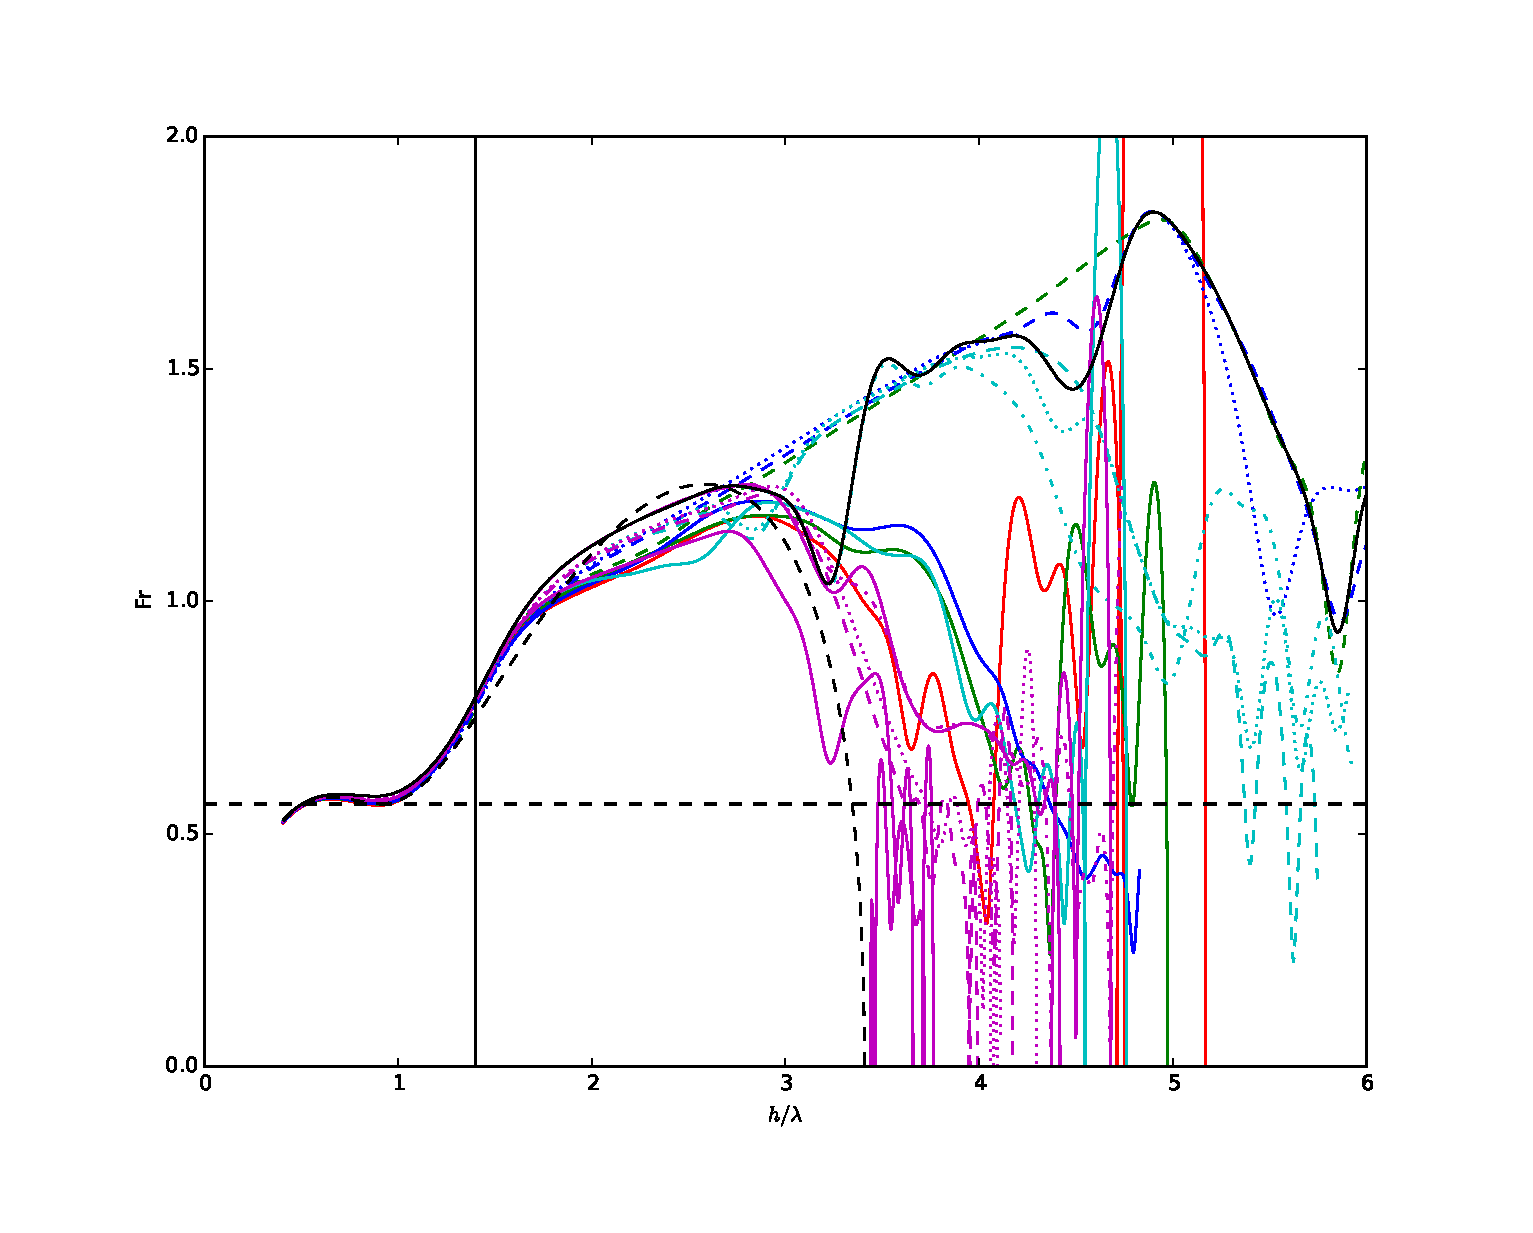
\includegraphics[width=0.66\columnwidth]{plts/Fr_long_walls}
\end{subfigure}
\begin{subfigure}[b]{0.66\columnwidth}
  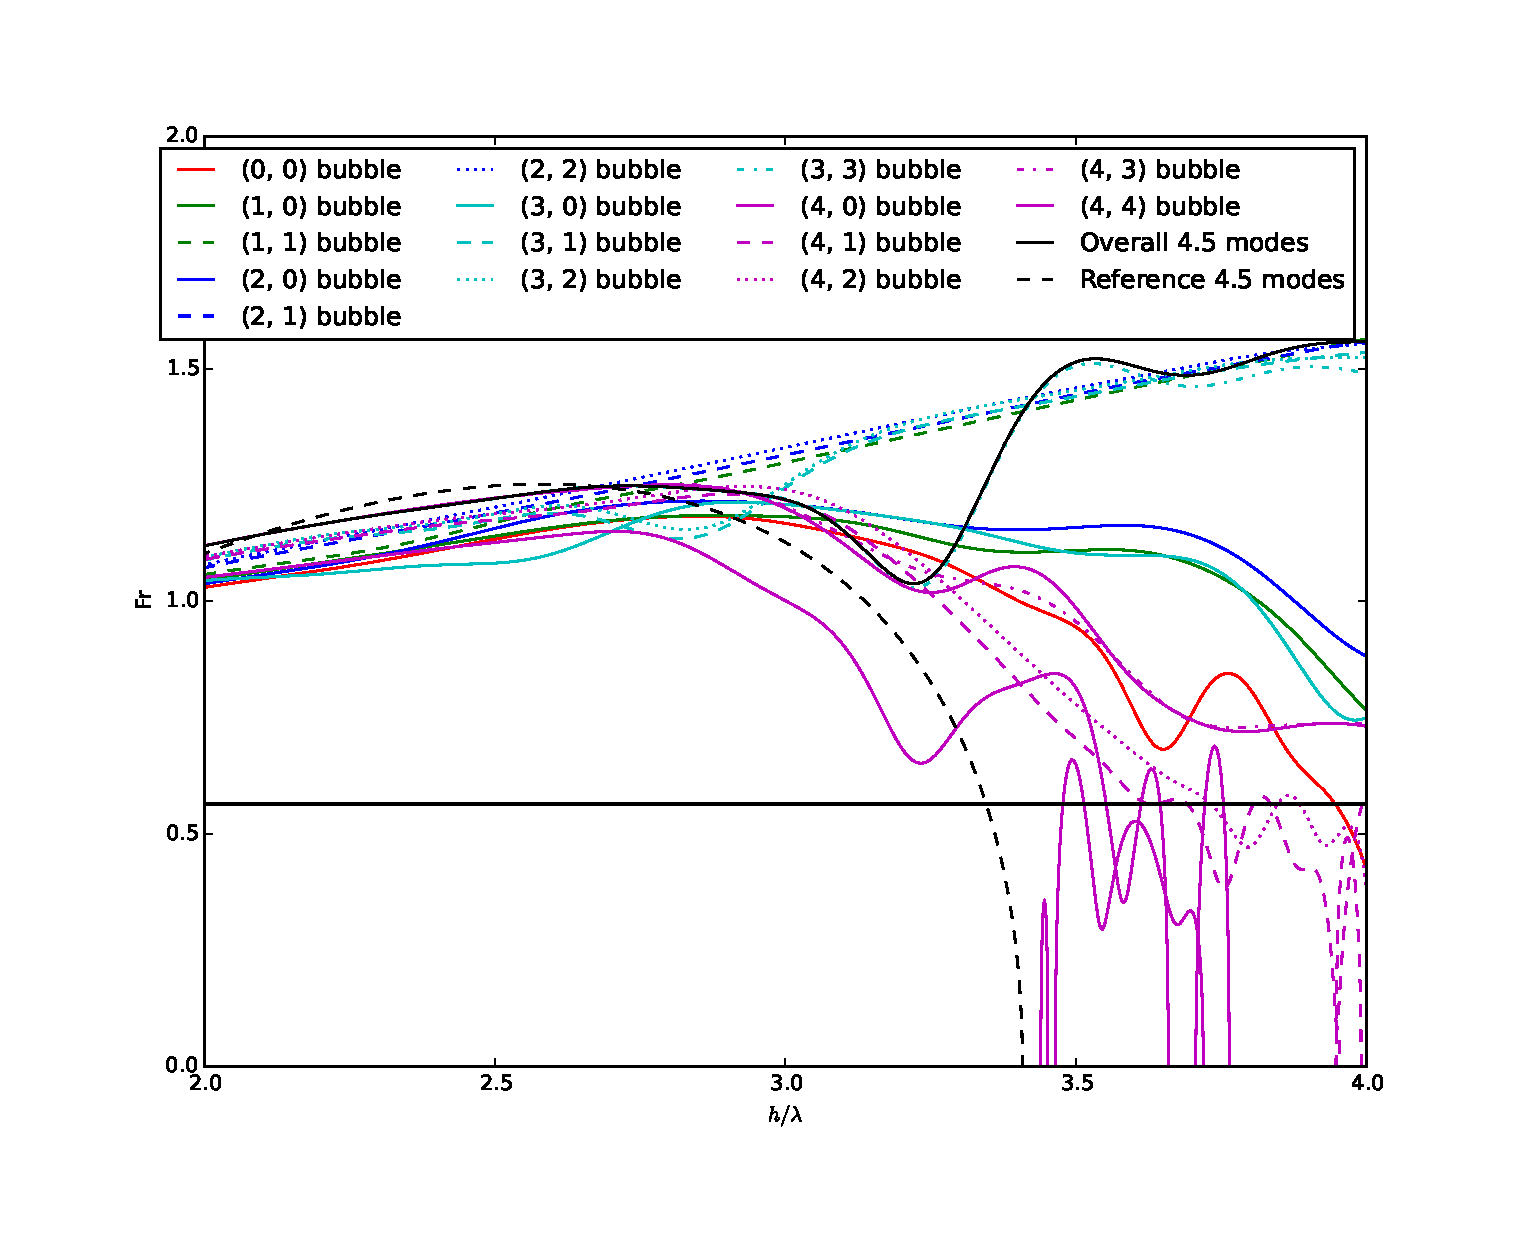
\includegraphics[width=0.66\columnwidth]{plts/Fr_long_walls_zoom1}
\end{subfigure}
\begin{subfigure}[b]{0.66\columnwidth}
  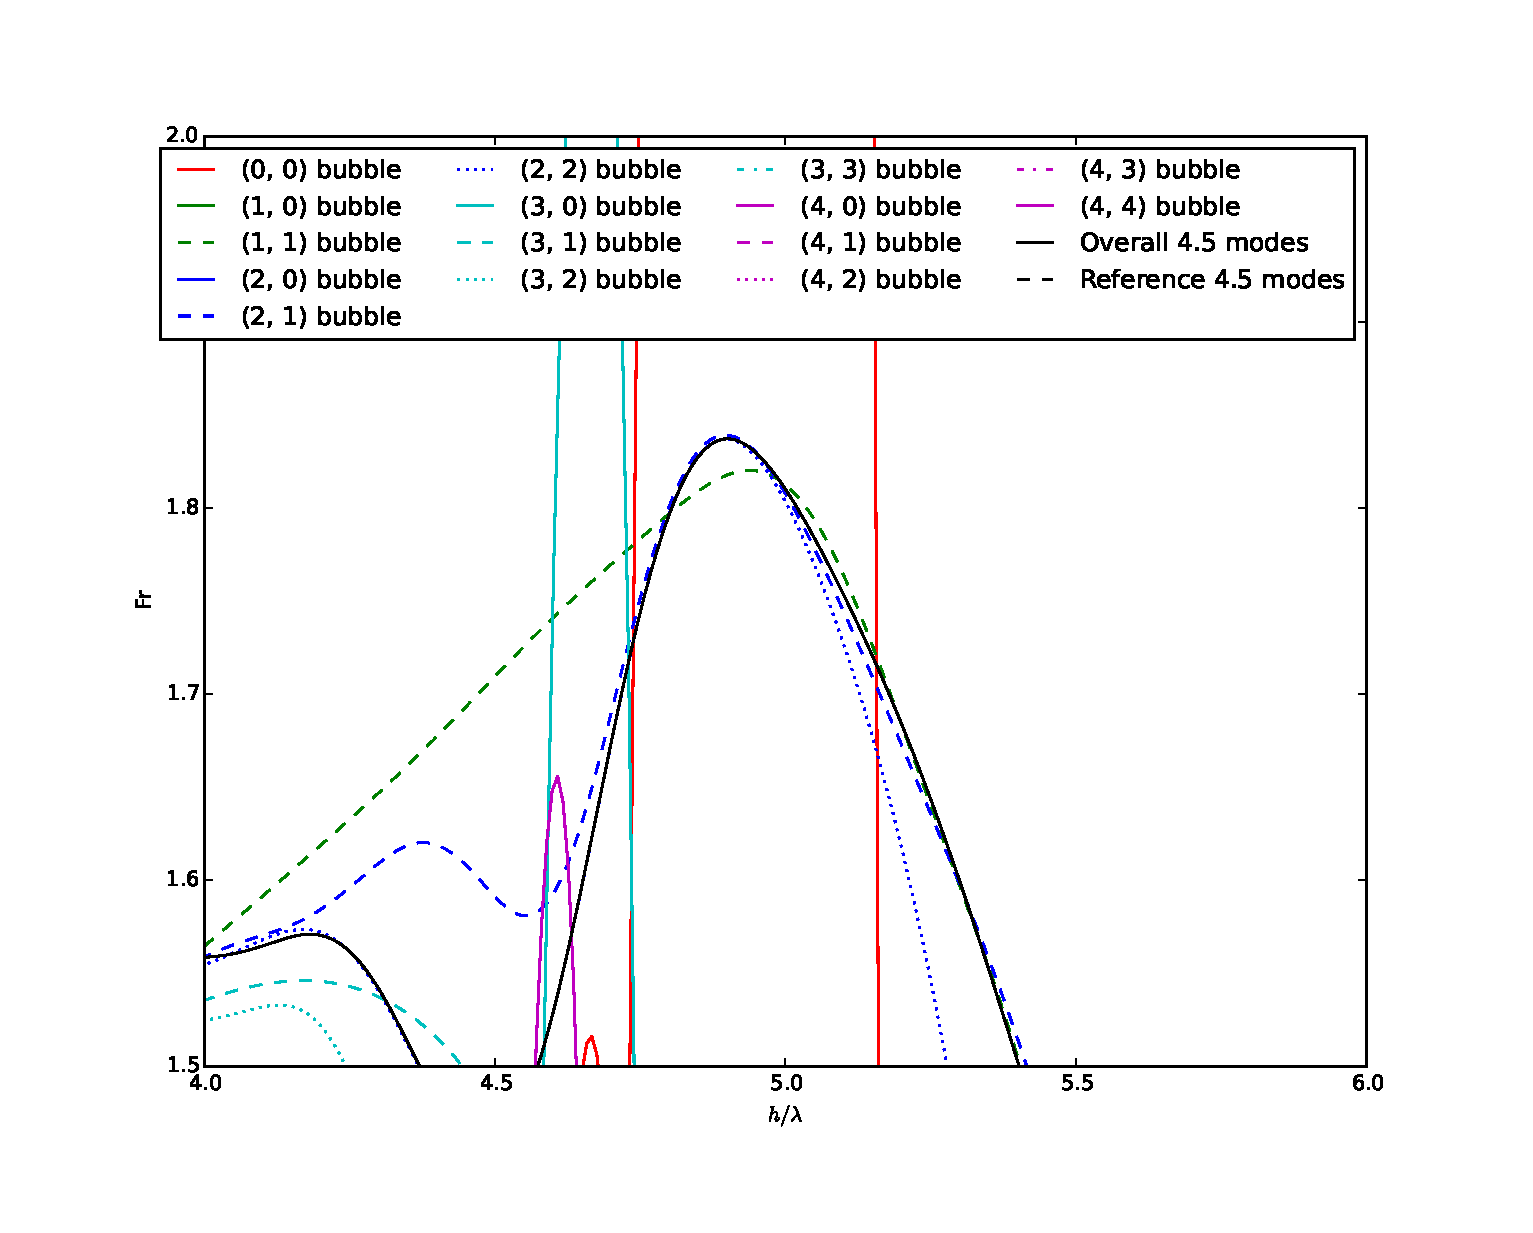
\includegraphics[width=0.66\columnwidth]{plts/Fr_long_walls_zoom2}
\end{subfigure}
\caption{ \flabel{long_wall_dynamics}
Froude number as a function of height, non-dimensionalized by the wavelength, by bubble in the 4.5 mode simulation with extended vertical extent.
Solid line is from the height defined as the maximum taken over the entire span-wise domain.
Dotted line is the periodic reference calculation.
The dotted horizontal line is positioned at Goncharov's theoretical value of $\pi^{-1/2}$~\cite{Goncharov2002}.
The solid vertical line marks the greatest bubble height reached in any of the experiments by Wilkinson and Jacobs~\cite{Wilkinson2007}.
}
\end{figure*}


The 4.5 mode simulation was repeated with twice the vertical extent and simulation time.
Additionally, the Schmidt number was increased from 1 to 3.5 to reduce late-time mixing not present in high Schmidt number experiments.
\fref{long_dynamics} compares the short unit-Schmidt and long moderate-Schmidt trajectories, which are widely in agreement.
The reduction in bubble acceleration around aspect ratio $h/\lambda = 2$ is present in both the short and the long simulations, so it is unlikely to be due to the vertical domain boundaries.
It is not, however, present in the periodic calculation, so it could be a wall effect.

\fref{long_wall_dynamics} mimics \fref{froude_wall} but for the late-time case.
The periodic reference trajectory, calculated with the original domain size, rapidly decays after reaching a maximum around aspect ratio $h/\lambda = 2.5$ due to interactions with the top of the domain.
Its maximum Froude number is around 1.2, consistent with previous calculations.
The central bubbles in the extended late-time run continue to experience constant acceleration past aspect ratio 3 and Froude number 1.2, with the $(1,1)$ bubble continuing to aspect ratio 5 and Froude number 1.8.

The decay of the velocity of the periodic reference bubble around $h/\lambda = 2.5$ suggests the late-time simulations would interact with the top boundary around $h/\lambda = 5$.
In fact, this is exactly when the $(1,1)$ and $(2,2)$ bubbles begin to decay.
However, the bubbles closer to the boundaries break down much earlier.
The $(4,4)$ bubble, for example, reaching maximum Froude number around $h/\lambda = 2.75$.
We can infer that the wall lift that drives the boundary bubbles into the interior bubbles destroys the periodic ordering.
It is not clear if the decay of the interior bubbles at $h/\lambda = 5$ is due to the top boundary or the wall lift destroying the periodic ordering.

\subsubsection{Secondary flow}

\begin{figure*}
\begin{subfigure}[b]{0.66\columnwidth}
  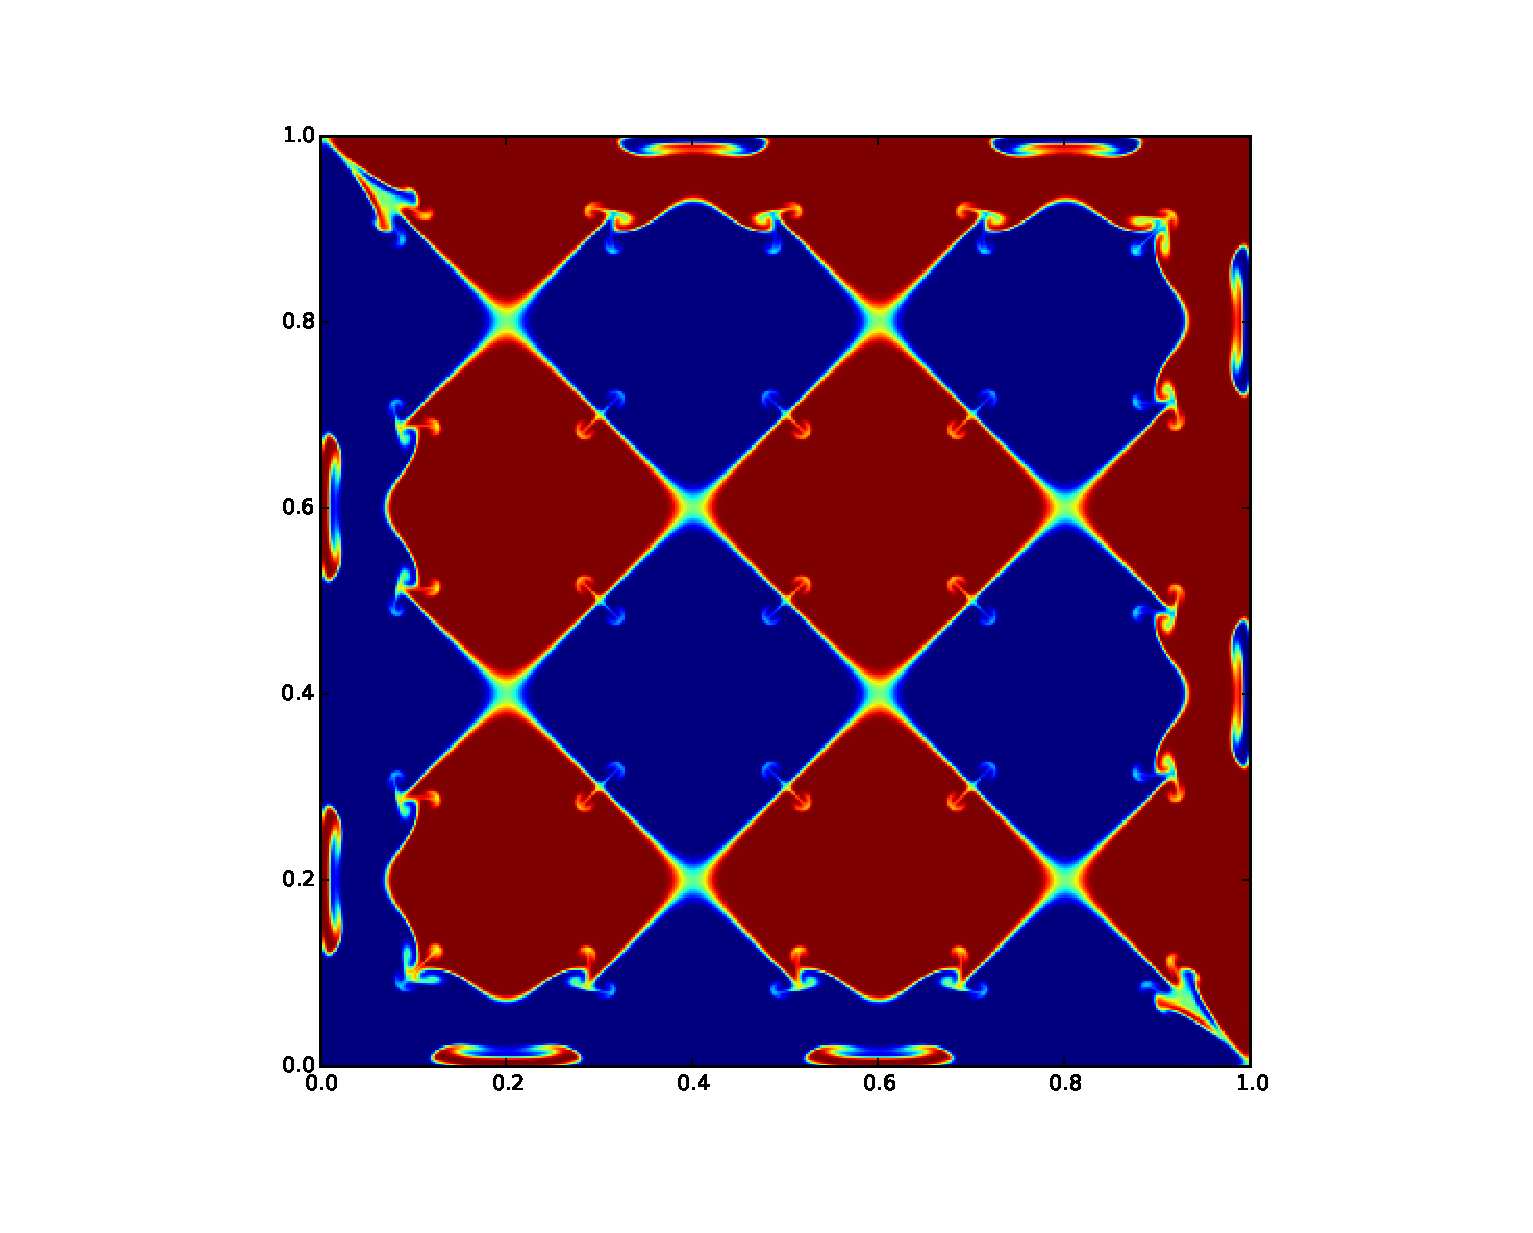
\includegraphics[width=0.66\columnwidth]{figs/scalar-25-20}
\end{subfigure}
\begin{subfigure}[b]{0.66\columnwidth}
  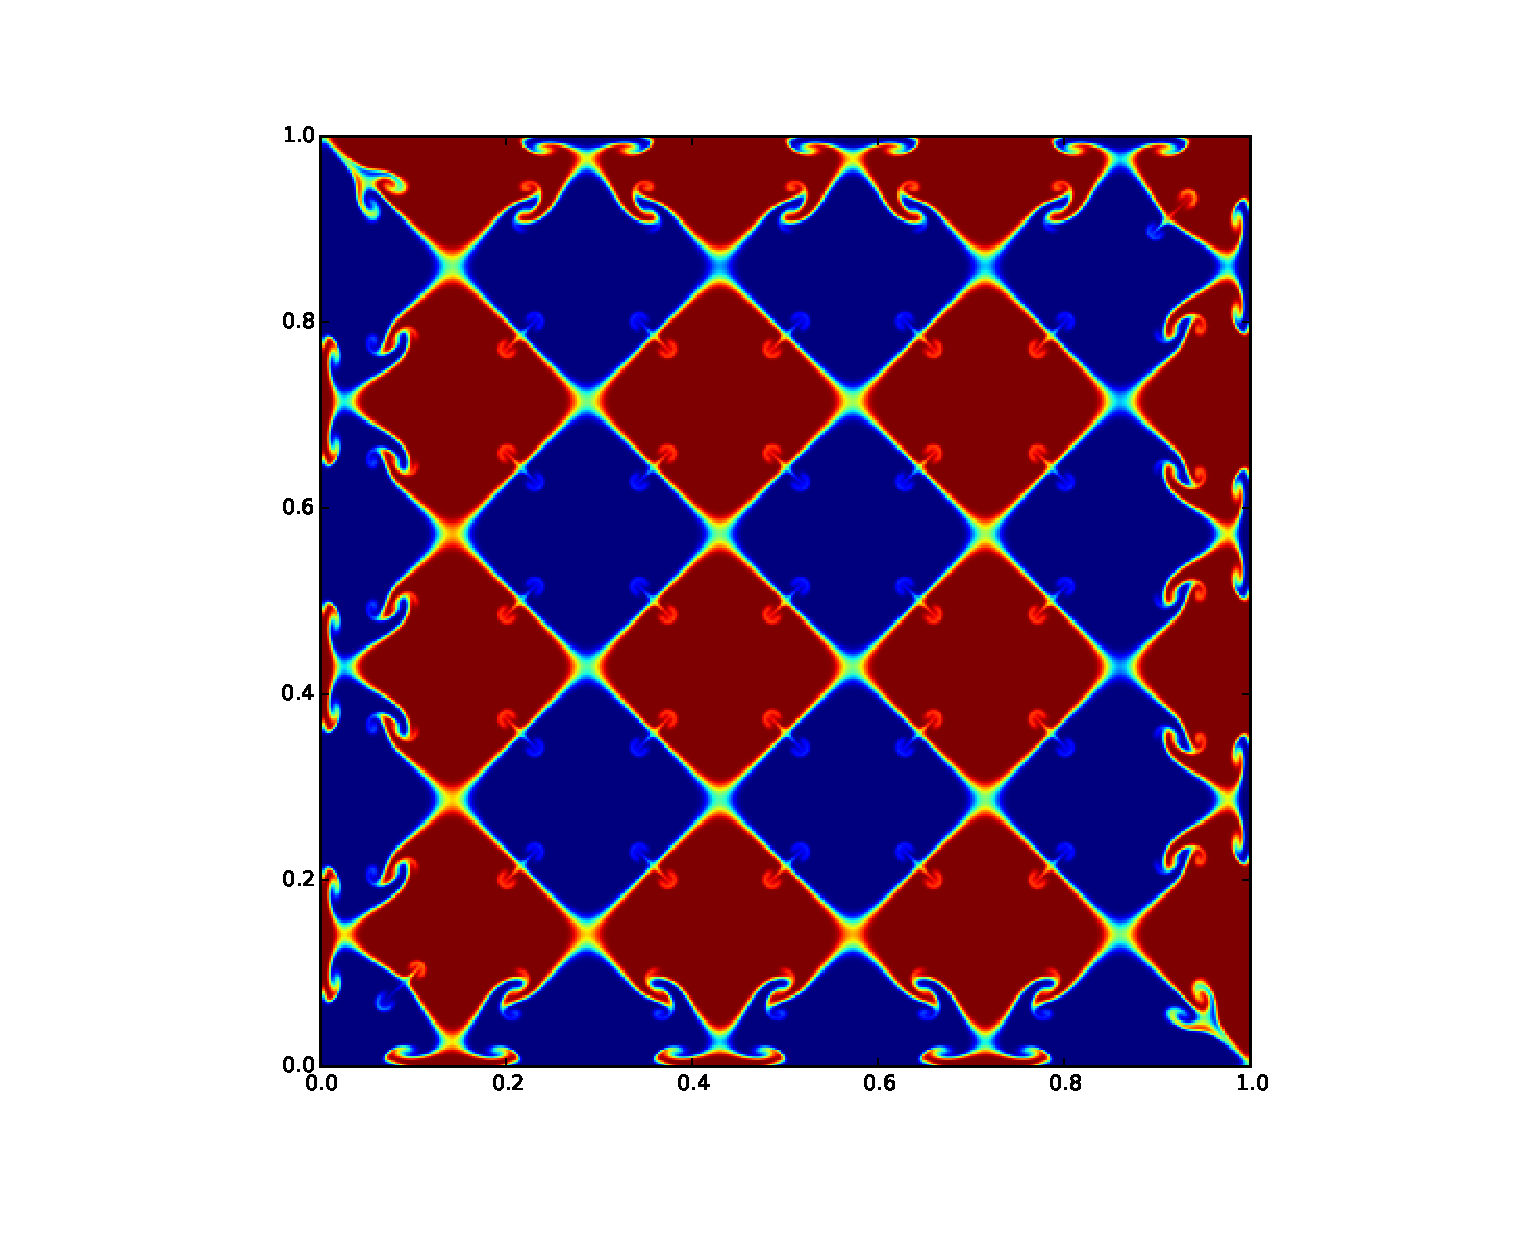
\includegraphics[width=0.66\columnwidth]{figs/scalar-35-20}
\end{subfigure}
\begin{subfigure}[b]{0.66\columnwidth}
  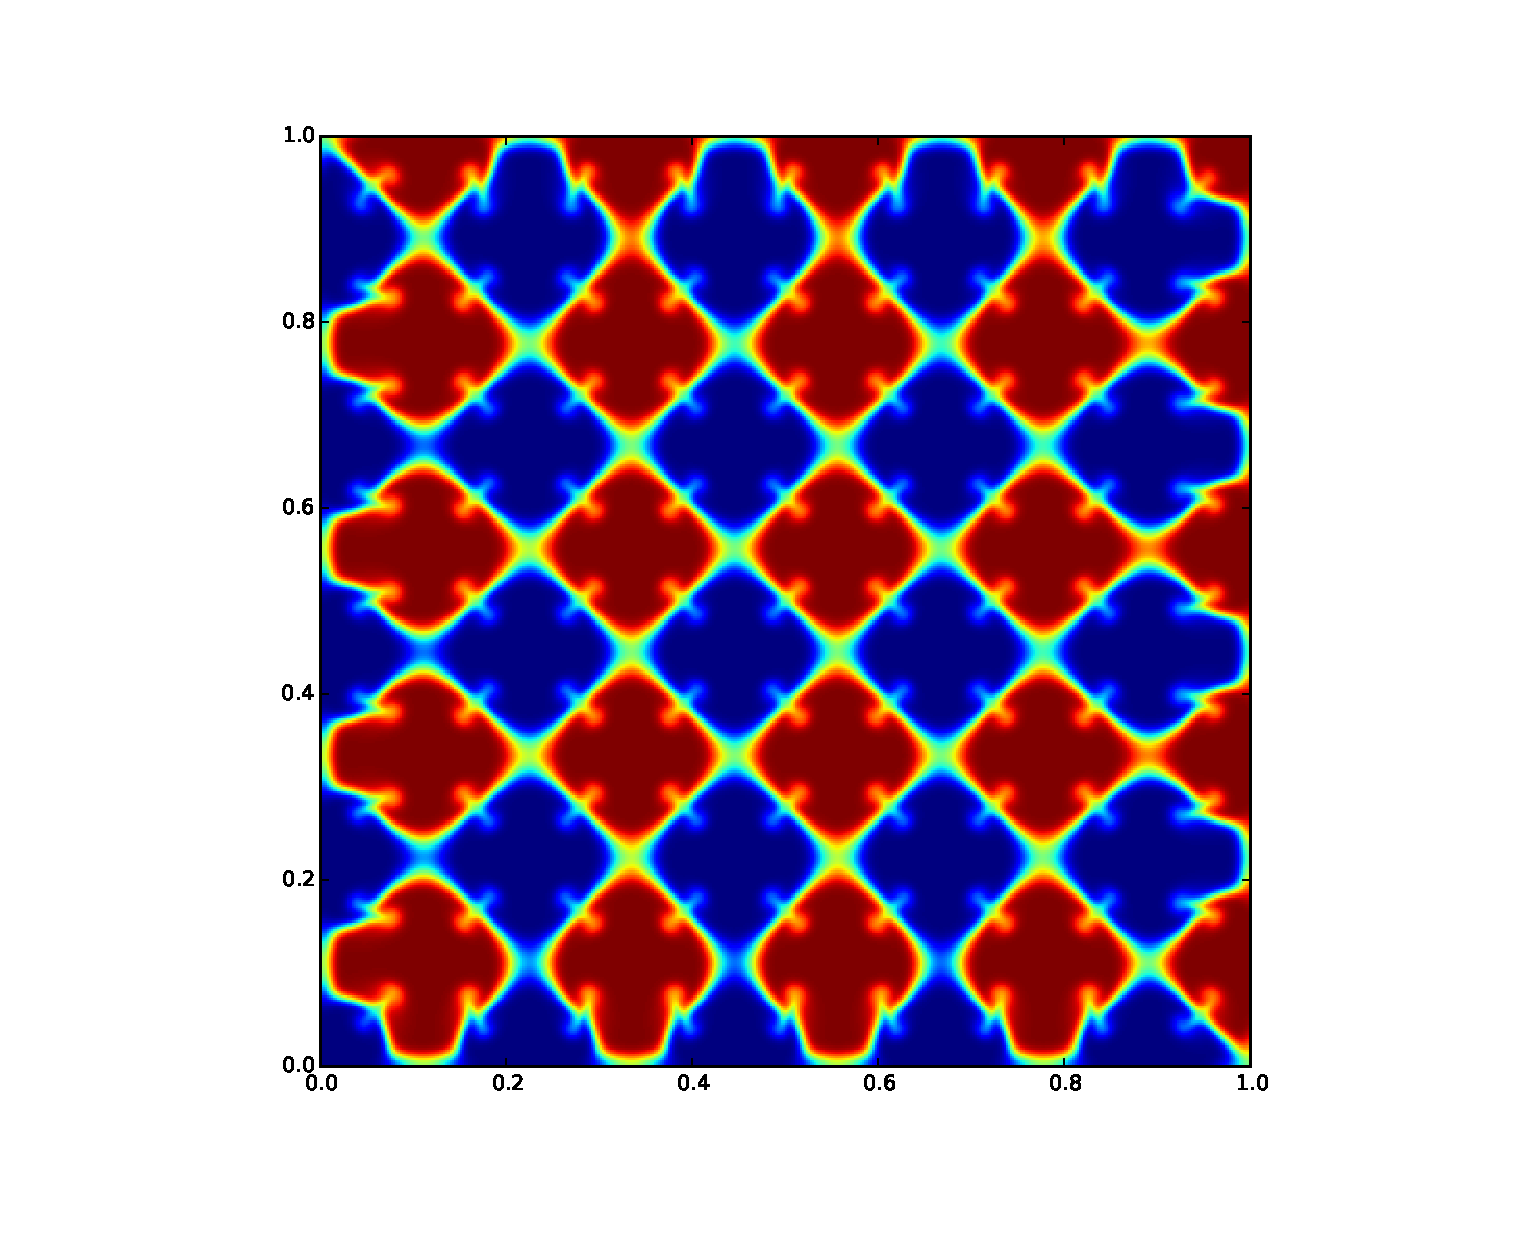
\includegraphics[width=0.66\columnwidth]{figs/scalar-45-20}
\end{subfigure}
\caption{ \flabel{phixy}
Scalar field in the horizontal mid-plane for 2.5, 3.5, and 4.5 mode simulations.
}
\end{figure*}



\begin{figure*}
\begin{subfigure}[b]{0.66\columnwidth}
  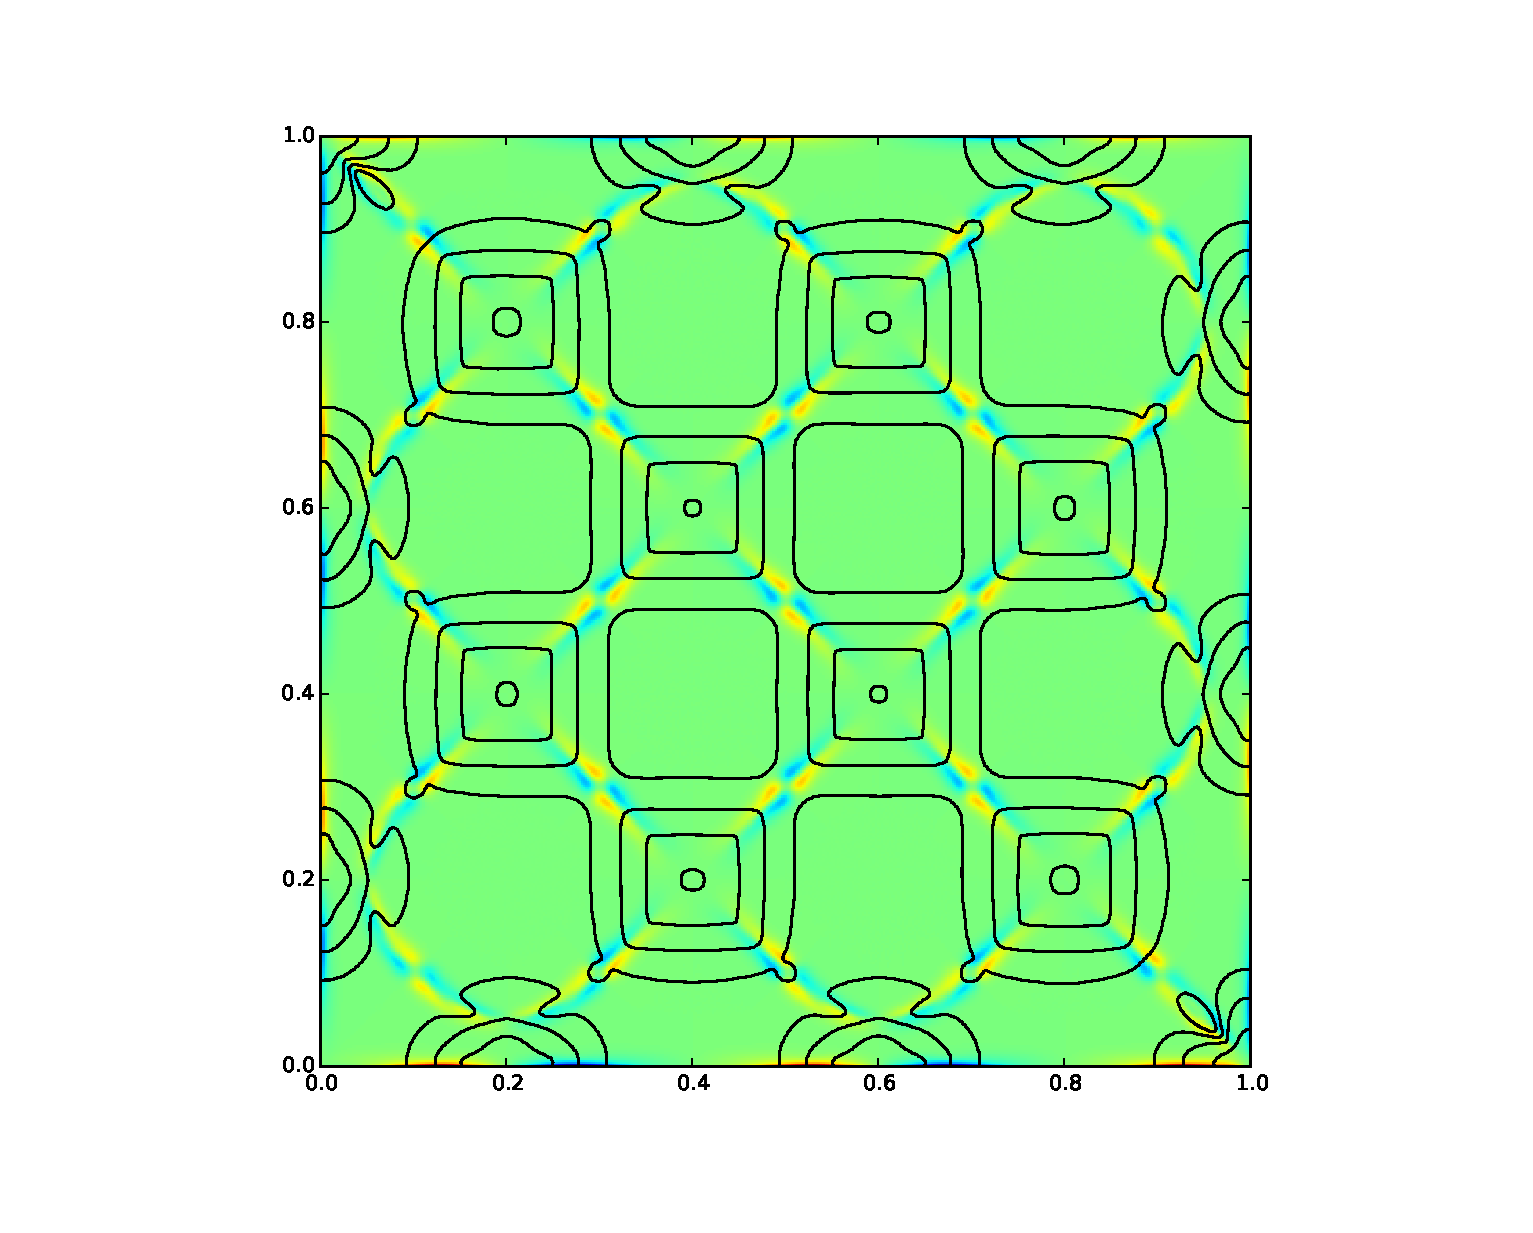
\includegraphics[width=0.66\columnwidth]{figs/vorticity-25-10}
\end{subfigure}
\begin{subfigure}[b]{0.66\columnwidth}
  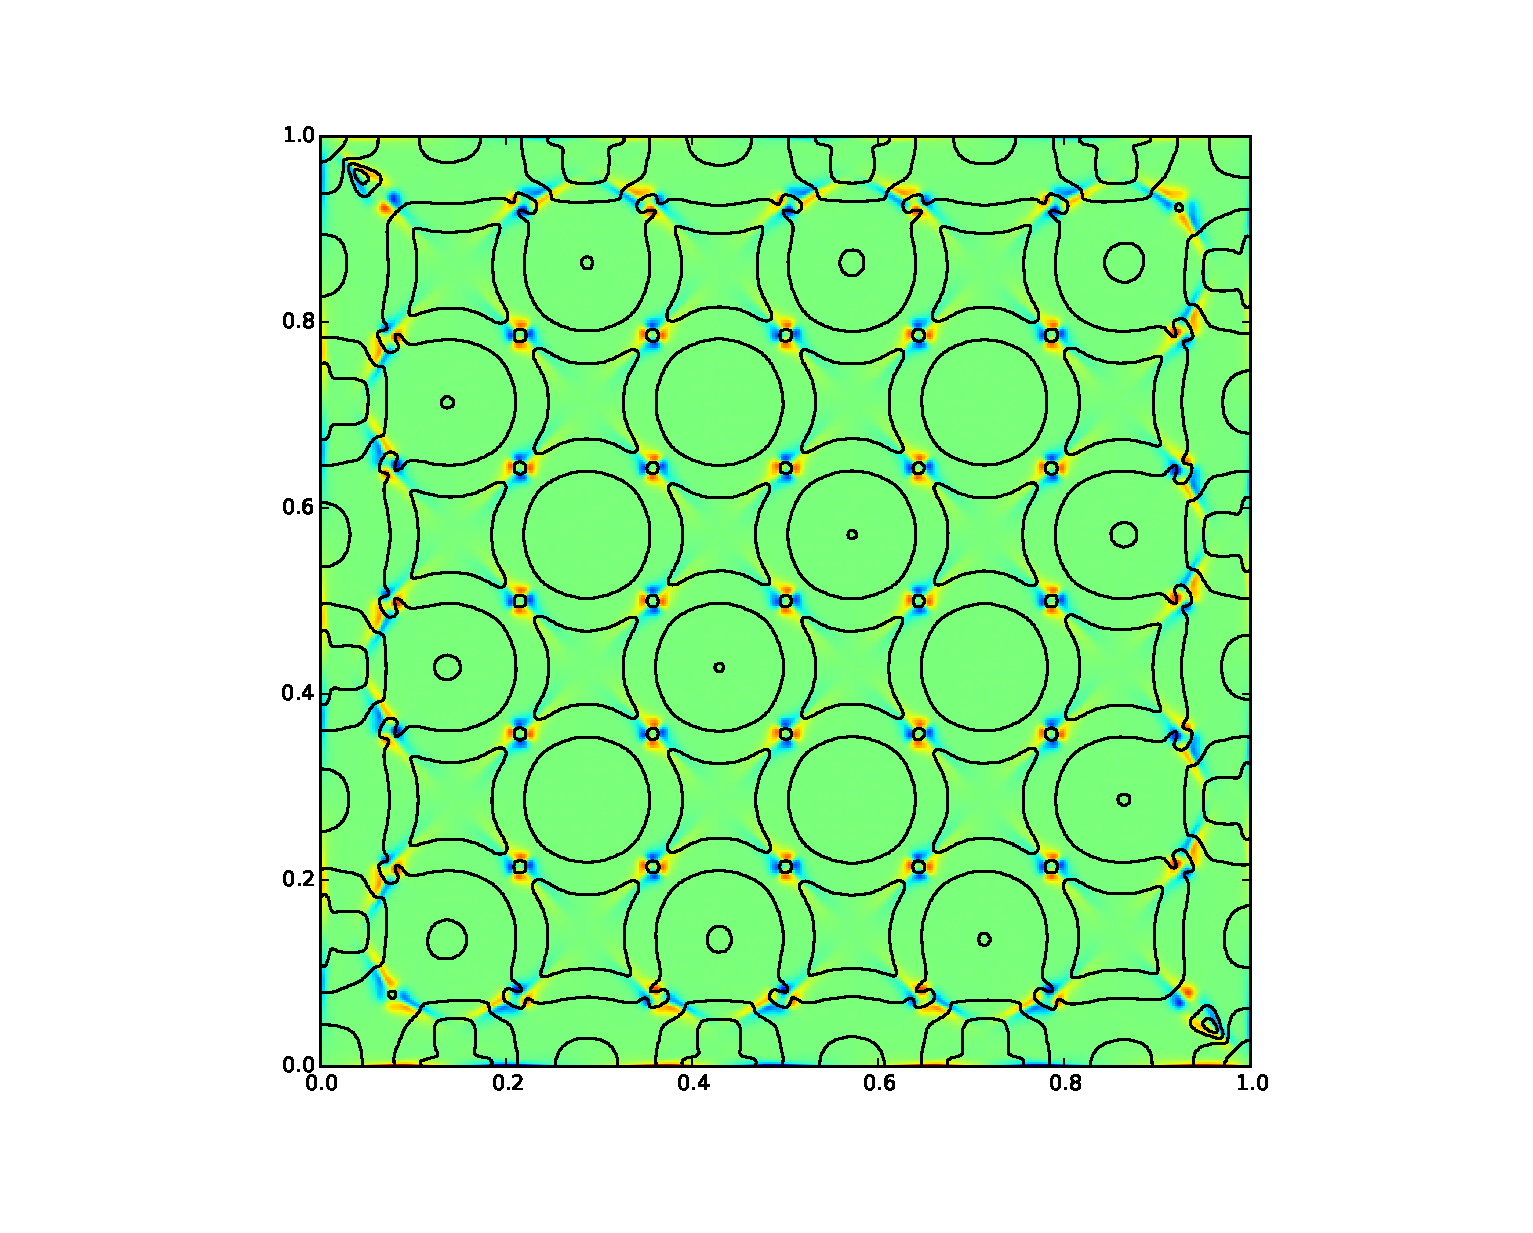
\includegraphics[width=0.66\columnwidth]{figs/vorticity-35-10}
\end{subfigure}
\begin{subfigure}[b]{0.66\columnwidth}
  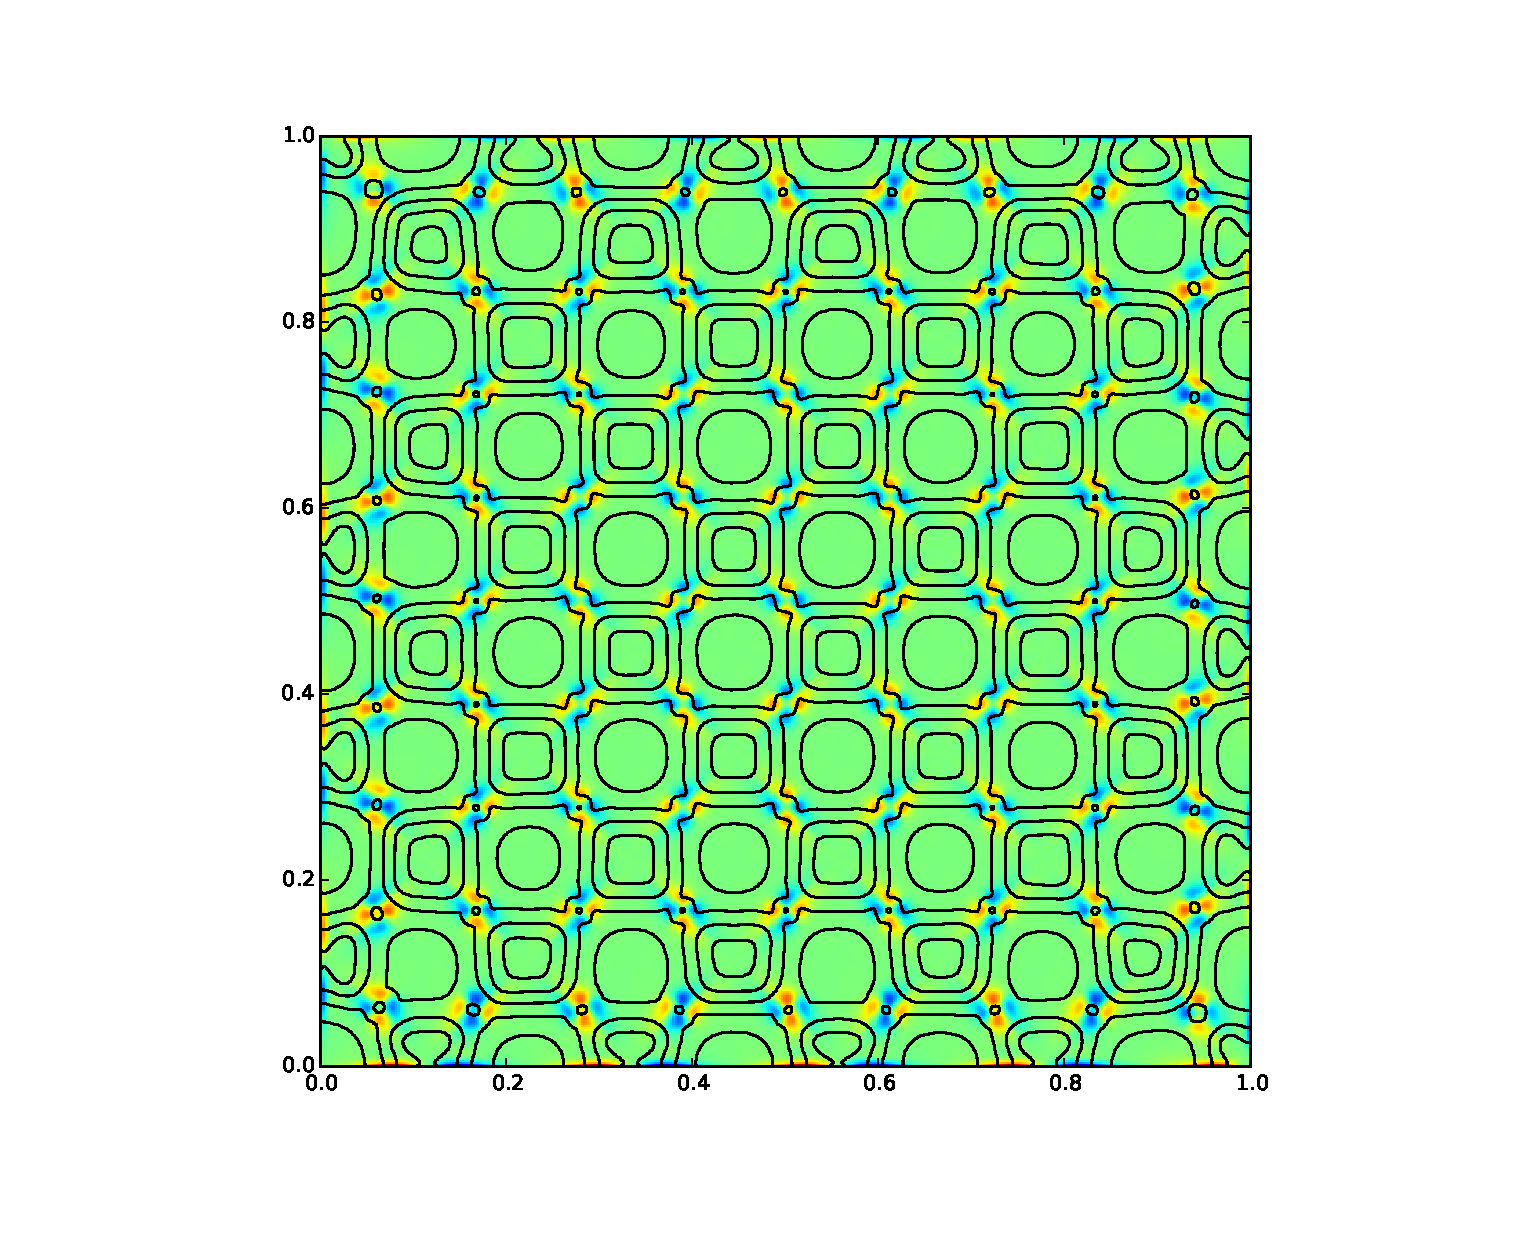
\includegraphics[width=0.66\columnwidth]{figs/vorticity-45-10}
\end{subfigure}
\caption{ \flabel{secondary}
Secondary flow in the horizontal mid-plane.
Background color is the vertical component of the vorticity.
Contours are lines of constant pressure.
}
\end{figure*}

\begin{figure*}
\begin{subfigure}[b]{0.66\columnwidth}
  \includegraphics[width=0.66\columnwidth]{figs/dynamic_pressure-25-10}
\end{subfigure}
\begin{subfigure}[b]{0.66\columnwidth}
  \includegraphics[width=0.66\columnwidth]{figs/dynamic_pressure-35-10}
\end{subfigure}
\begin{subfigure}[b]{0.66\columnwidth}
  \includegraphics[width=0.66\columnwidth]{figs/dynamic_pressure-45-10}
\end{subfigure}
\caption{ \flabel{dynamic}
Dynamic pressure in the horizontal mid-plane.
}
\end{figure*}


In addition to the bubble height and vertical slices in the diagonal plane, we observe the horizontal mid-plane.
The span-wise scalar field, $\phi(x,y,0)$, exhibits plume structures that penetrate the bubble faces, as seen in \fref{phixy}.
The cause of these plumes is advection by secondary flows, as seen in \fref{secondary}.
Overlaying the pressure with the span-wise velocity reveals it to be secondary flow of the first kind: secondary flow due to span-wise pressure gradients.
The span-wise pressure gradient comes from the dynamic pressure of the rising and falling bubbles and spikes, in contrast to the stationary points at their interfaces.

The secondary flow advects mixed fluid from the interface into the centers of the bubbles and spikes.
Enhanced mixing reduces the effective Atwood number of the bubbles and spikes, but the magnitude of this effect is not clear.
As a secondary flow of the first kind, this mixing mode is present even at low Reynolds numbers.



\section{Conclusions} \slabel{concs}

The simulations described here reproduce the growth rate, stagnation velocity, and re-acceleration of the low-Atwood single mode Rayleigh Taylor instability for three experimental runs by Wilkinson and Jacobs.
These reproductions inspire confidence not only in the NekBox code, but also in the Boussinesq approximation for $A = 0.15$ and the low-Schmidt approximation.

In wall-bounded flows, the bubbles and spikes nearest to the no-slip boundaries experience lift and drag forces that slow their non-linear growth and push them towards their inner neighbors.
There is an additional effect due to the finite domain breaking one of the 4-fold symmetries from the purely periodic problem.
In the wall-bounded initial condition, one corner of the domain has an excess of bubbles while the opposite has an excess of spikes.
This sets up a long-wavelength mode across the diagonal that encourages bubble growth in one corner and discourages it in the other.

Ultimately, the bubble-bubble and spike-spike collisions may destroy the single-mode ordering of the flow at aspect ratio 5, but the onset of velocity decay may alternatively be due to the upper boundary.
If the decay is due to collisions, it would limit the use of wall-bounded flows as proxies for periodic flows to moderate aspect ratios.
The ability of wall-bounded flows to approximate periodic ones at high aspect ratio warrants further study.

In addition to causing collisions, the growing boundary layer squeezes the flow in the span-wise direction, accelerating it past its fully-periodic trajectory in the stagnation and re-acceleration phases.

The inner bubbles experience near constant acceleration from aspect ratio 2 to aspect ratio 5, with a maximum Froude number of 1.8.
This contrasts results by Ramaprabhu et al.~\cite{Ramaprabhu2012} that show saturation post-reacceleration at $\text{Fr} \approx 1$.
The saturation could be explained by excess mixing or the finite size of the domain, which extends to $h/\lambda = 6$ in their case and $9$ in ours.
Alternatively, the acceleration could be artificially sustained by the wall lift force pushing the boundary bubbles into the interior ones.

Single-mode Rayleigh-Taylor flows develop span-wise pressure gradients with local minima in bubble and spike centers and local maxima in bubble and spike corners.
The pressure drives secondary flows of the first kind in the form of vortex quads centered on bubble-spike interface centers.
These span-wise flows mix the fluid across otherwise laminar interfaces, perturbing the scalar profiles.

\section{Acknowledgements}

M. H. is grateful for useful conversations with Jeffrey Jacobs, Robert Roser, Aleksandr Obabko, Elia Merzari, Oana Marin, and Elizabeth Hicks.

M. H. acknowledges support from the Department of Energy Computational Science graduate fellowship.
This research used resources of the Argonne Leadership Computing Facility, which is a DOE Office of Science User Facility supported under Contract DE-AC02-06CH11357.




\chapter{Conclusions}

\section{New model for low-Atwood single mode}

\section{Validation of DNS}

\section{Importance of Schmidt number}

\section{Open questions}

 % Conclusion

% Format a LaTeX bibliography
\makebibliography

% Figures and tables, if you decide to leave them to the end
%\input{figure}
%\input{table}

\end{document}


